%% Henrik Andersson
%% 2005-04-14
\documentclass{scrartcl}
\usepackage{booktabs}
\usepackage{graphicx,color}
\usepackage{natbib}
\usepackage{fancyhdr}
\usepackage{amsmath}
\usepackage{makeidx}
\makeindex
\usepackage[colorlinks]{hyperref}



\pagestyle{fancy}

% \VignettePackage{femmeR}
% \VignetteIndexEntry{An R companion to FEMME}

\title{\Rcode{femmeR} -- An \R{} companion to FEMME}
\author{Henrik Andersson \and Andreas Hofmann \and Karline Soetaert}

\newcommand{\femmecode}[1]{\texttt{\textcolor{red}{#1}}}
\newcommand{\Rcode}[1]{\texttt{\textcolor{blue}{#1}}}
\newcommand{\R}{\textsf{R}}
\newcommand{\Fortran}{\textsc{Fortran}}
\newcommand{\fn}[1]{\texttt{#1}\index{#1}\\}


%%% -----------------------------------------------------------------
\usepackage{/data/han/local/lib/R/share/texmf/Sweave}
\begin{document}
 
\maketitle
\setcounter{tocdepth}{1}

\begin{abstract}
  \Rcode{femmeR} is a package of functions mainly used to visualize
  output from the ecological modelling environment FEMME developed by
  \citet{soetaert00b}.
\end{abstract}


\tableofcontents
\setkeys{Gin}{width=0.6\textwidth}

\newpage

\noindent \textsf{This document explains the use of \Rcode{femmeR}, however if
  you are not familiar with \R{} a brief guide is found in Appendix~\ref{sec:short-introduction-r}}

\section{Steady state 1D}

To process the output from a steady-state application, read the file
and plot the results,\index{read.st1} \index{plot.st1}


\begin{Schunk}
\begin{Sinput}
> test <- read.st1("ENHDIFF1.ST1")
> plot(test)
\end{Sinput}
\end{Schunk}
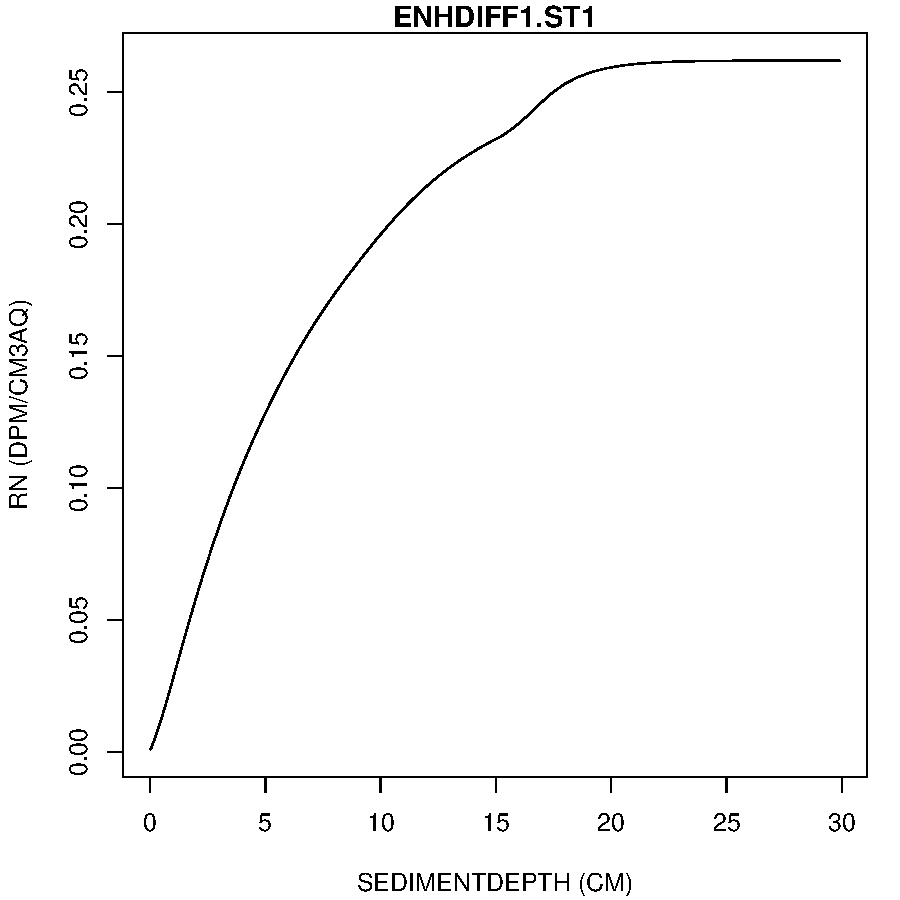
\includegraphics{figures/f-002}

The default plot command chooses the first and second variable in the
output file, to plot different variables, change \Rcode{xvari} or
\Rcode{yvari} and reverse an axis using e.g. \Rcode{rev="y"}, and
change the default labels. 

\begin{Schunk}
\begin{Sinput}
> plot(test, xvari = 2, yvari = 1, rev = "y", xlab = "Radon (dpm/dm3)")
\end{Sinput}
\end{Schunk}
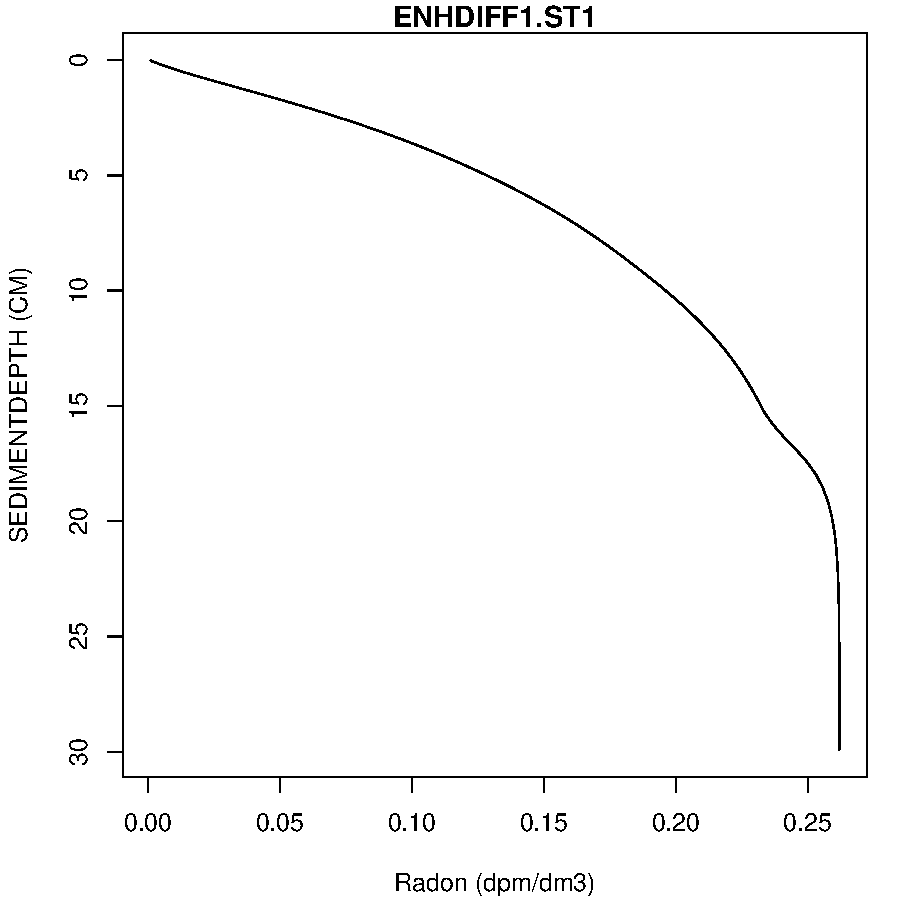
\includegraphics{figures/f-003}

Adding observed values to the output is very useful to check the model
performance,

\begin{Schunk}
\begin{Sinput}
> test.obs <- read.obs("sep.obs")
> plot(test, xvari = 1, yvari = 2, rev = "y", obs = test.obs)
\end{Sinput}
\end{Schunk}
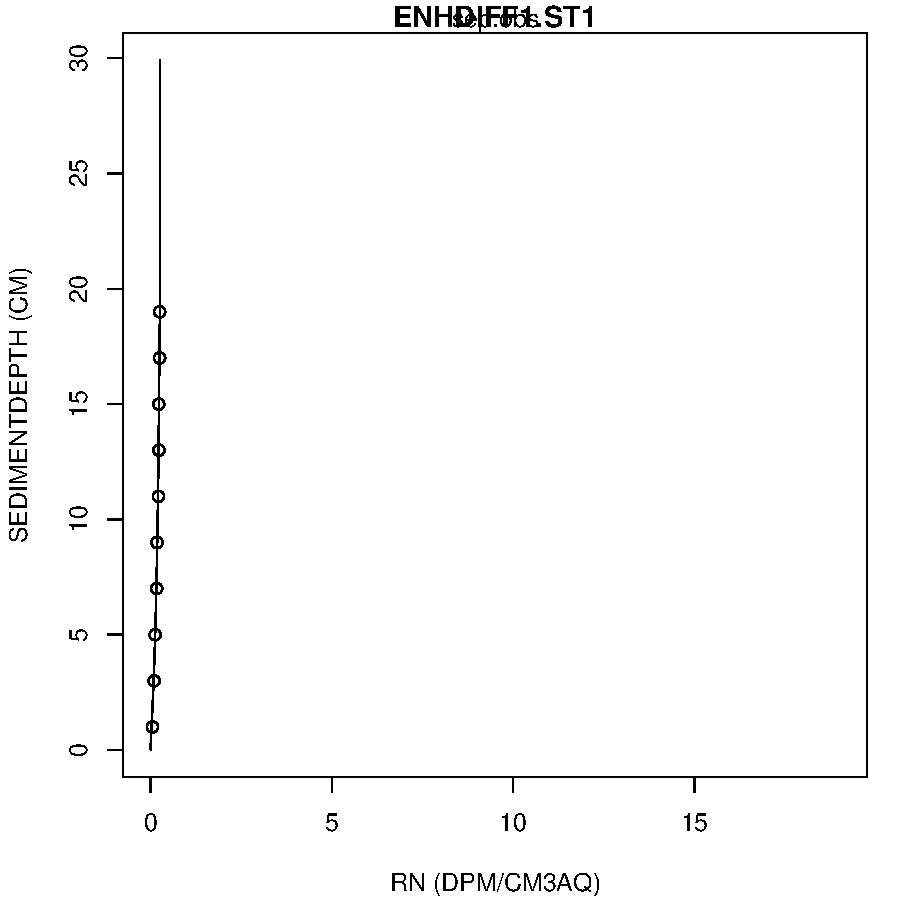
\includegraphics{figures/f-004}

\section{Time dependent 0-d}

Time dependent 0-d output are read and plotted in almost exactly the
same way as one-dimensional steady-state output. \index{read.o1} \index{plot.o1}

\begin{Schunk}
\begin{Sinput}
> test.o1 <- read.o1("DILUTIONIRRIGATION.O1")
> plot(test.o1, xvar = 1, yvar = 3)
\end{Sinput}
\end{Schunk}
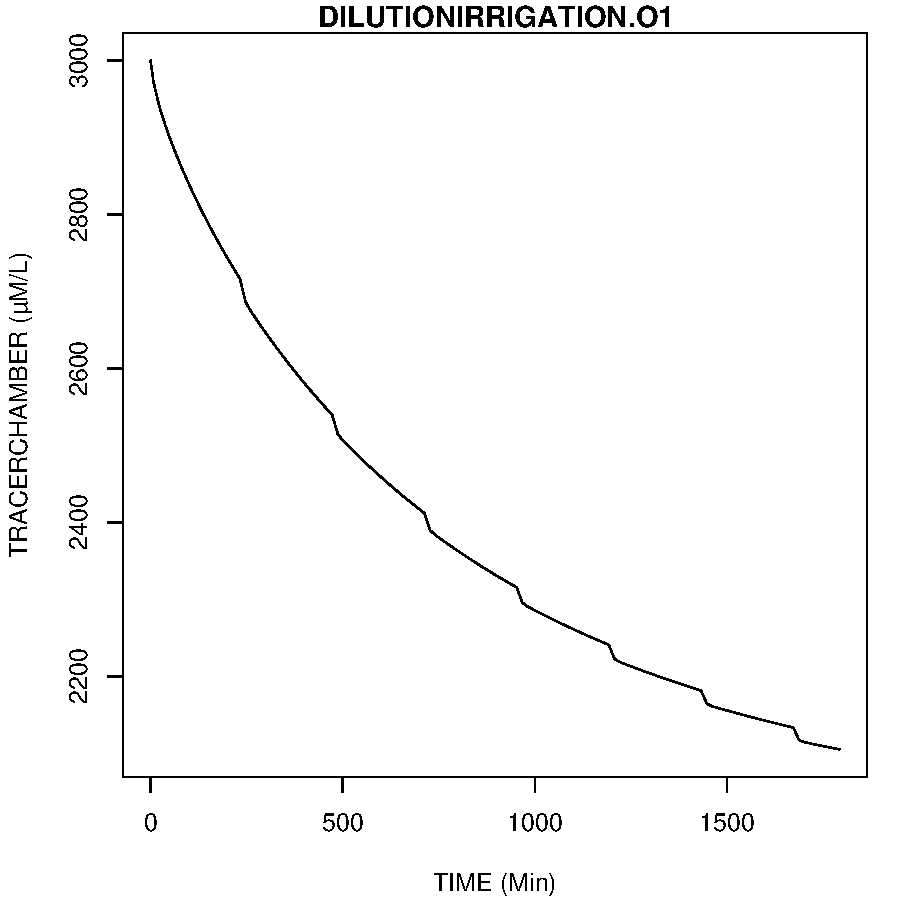
\includegraphics{figures/f-005}

Variable can be selected either using the number in which they appear
in the file or by a string with the variable name,

\begin{Schunk}
\begin{Sinput}
> plot(test.o1, xvari = "TIME", yvari = 3)
\end{Sinput}
\end{Schunk}
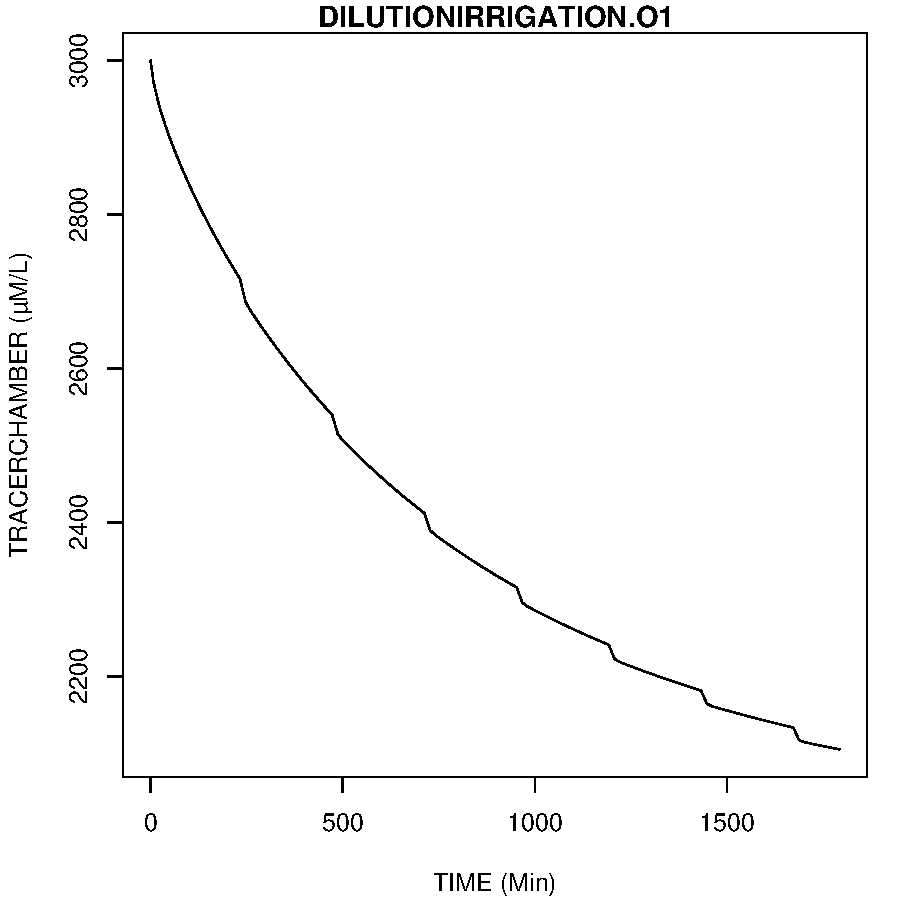
\includegraphics{figures/f-006}

If you don't know which variables you have, or simply forgot the
clever names you gave them:

\begin{Schunk}
\begin{Sinput}
> test.o1
\end{Sinput}
\begin{Soutput}
femmeR object of class o1
Filename: DILUTIONIRRIGATION.O1 

Variables
--------------------
1 TIME 
2 SURFACEMIXINGRATE 
3 TRACERCHAMBER 
4 TRACERCHAMBERINI 
5 TRACERFLUXSED 
6 TRACERDEEPFLUX 
7 INTEGRATEDTRACERCONCCHA 
8 INTEGRATEDTRACERCONCSED 
9 INTEGRATEDTRACERCONC 
10 VOLUMEREPLACED 
11 TRACERREMOVED 
12 CHAMBERVOLUME 
13 INTEGRATEDCONSUMPTION 
\end{Soutput}
\end{Schunk}

Plotting several variables at once is also possible, selecting a set
with e.g. \Rcode{yvari=c(3,5,8)} or \Rcode{yvari=2:5}, or using
the actual names of the variables, \Rcode{yvari=c("PH","CO2")}.

\begin{Schunk}
\begin{Sinput}
> plot(test.o1, xvar = 1, yvari = c(3, 5, 8, 10), main = "")
\end{Sinput}
\end{Schunk}
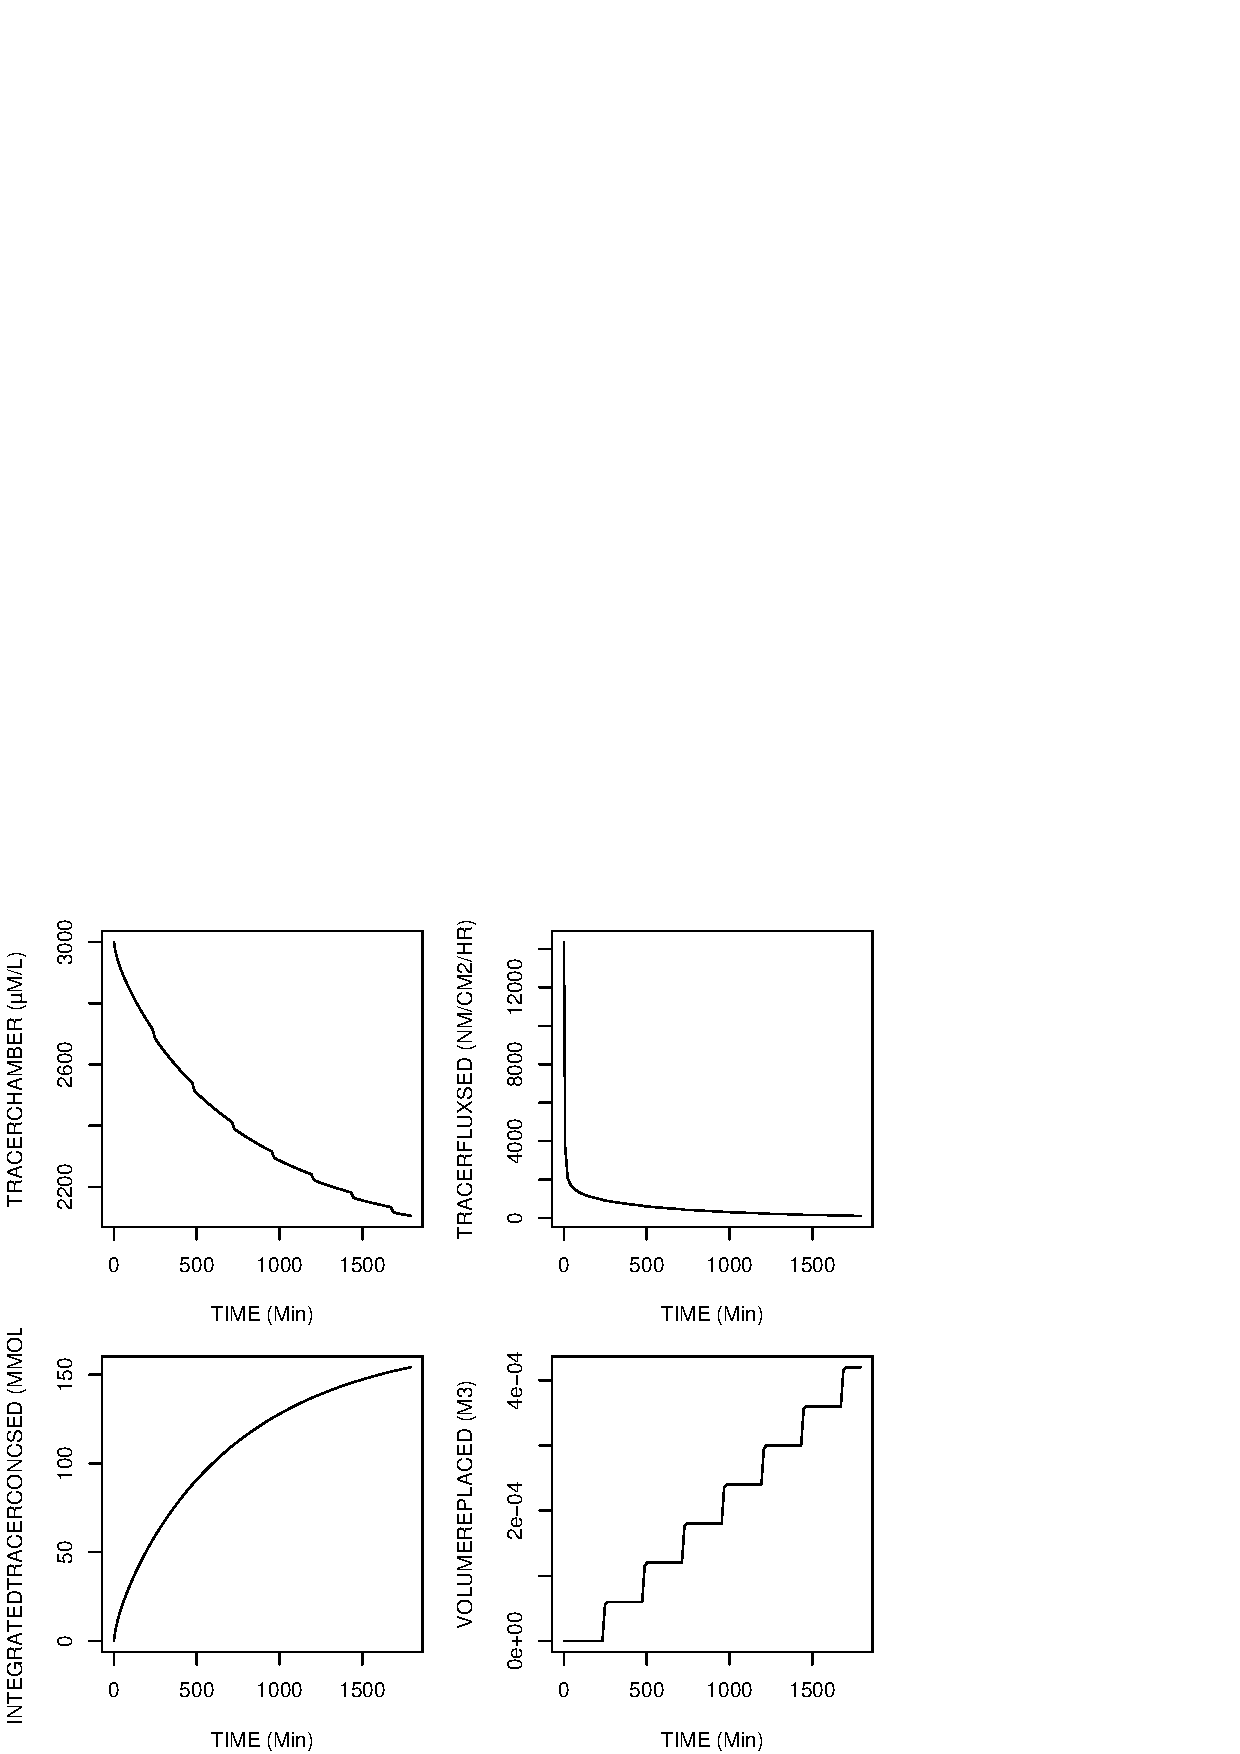
\includegraphics{figures/f-008}
\section{Time dependant 1-d}

Reading a file with data varying in space and time is done in the same
way as for other files. \index{read.o2} \index{plot.o2}

\begin{Schunk}
\begin{Sinput}
> test.o2 <- read.o2("BERG.O2")
\end{Sinput}
\end{Schunk}
Visualizing xyz data can be done in numerous ways, the simplest is to
use the function \Rcode{plot.o2}:

\begin{Schunk}
\begin{Sinput}
> plot(test.o2, zvari = 3, rev = "y")
\end{Sinput}
\end{Schunk}
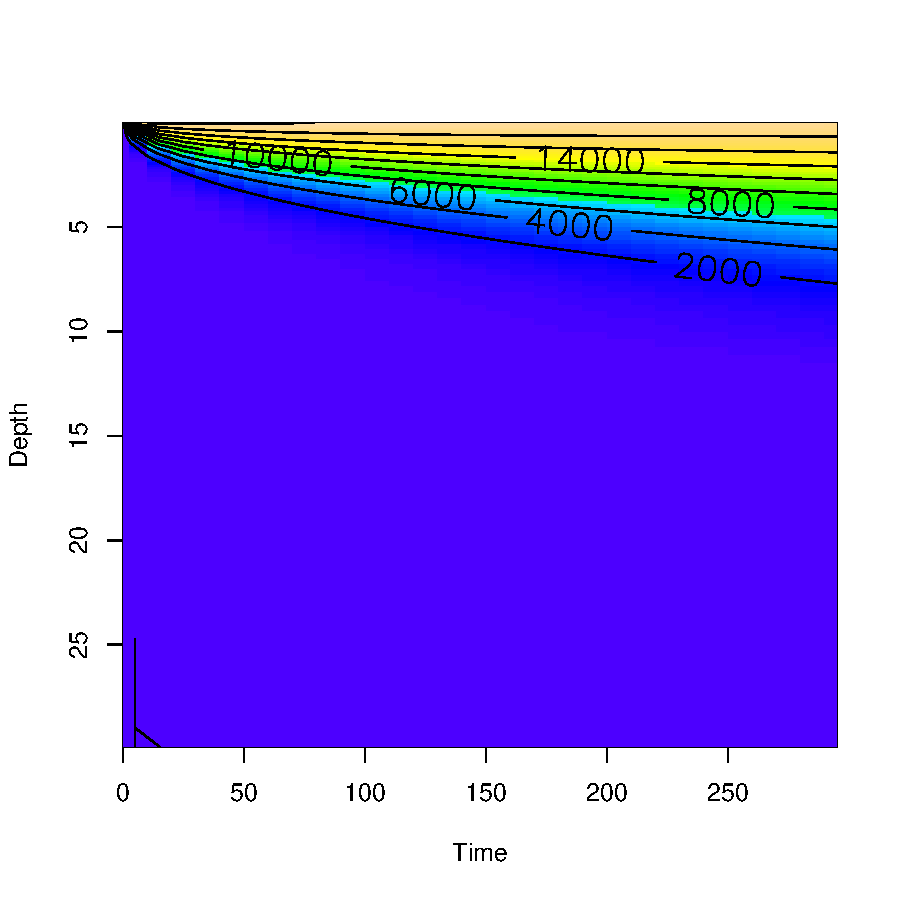
\includegraphics{figures/f-1Db}

As usual a number of options can be set, axis labels and contour lines
can be changed:
\begin{Schunk}
\begin{Sinput}
> plot(test.o2, zvari = 3, ylim = c(10, 0), ylab = "Depth (cm)", 
+     xlab = "Time (h)", linecol = "white", labcex = 1, lty = 2)
\end{Sinput}
\end{Schunk}
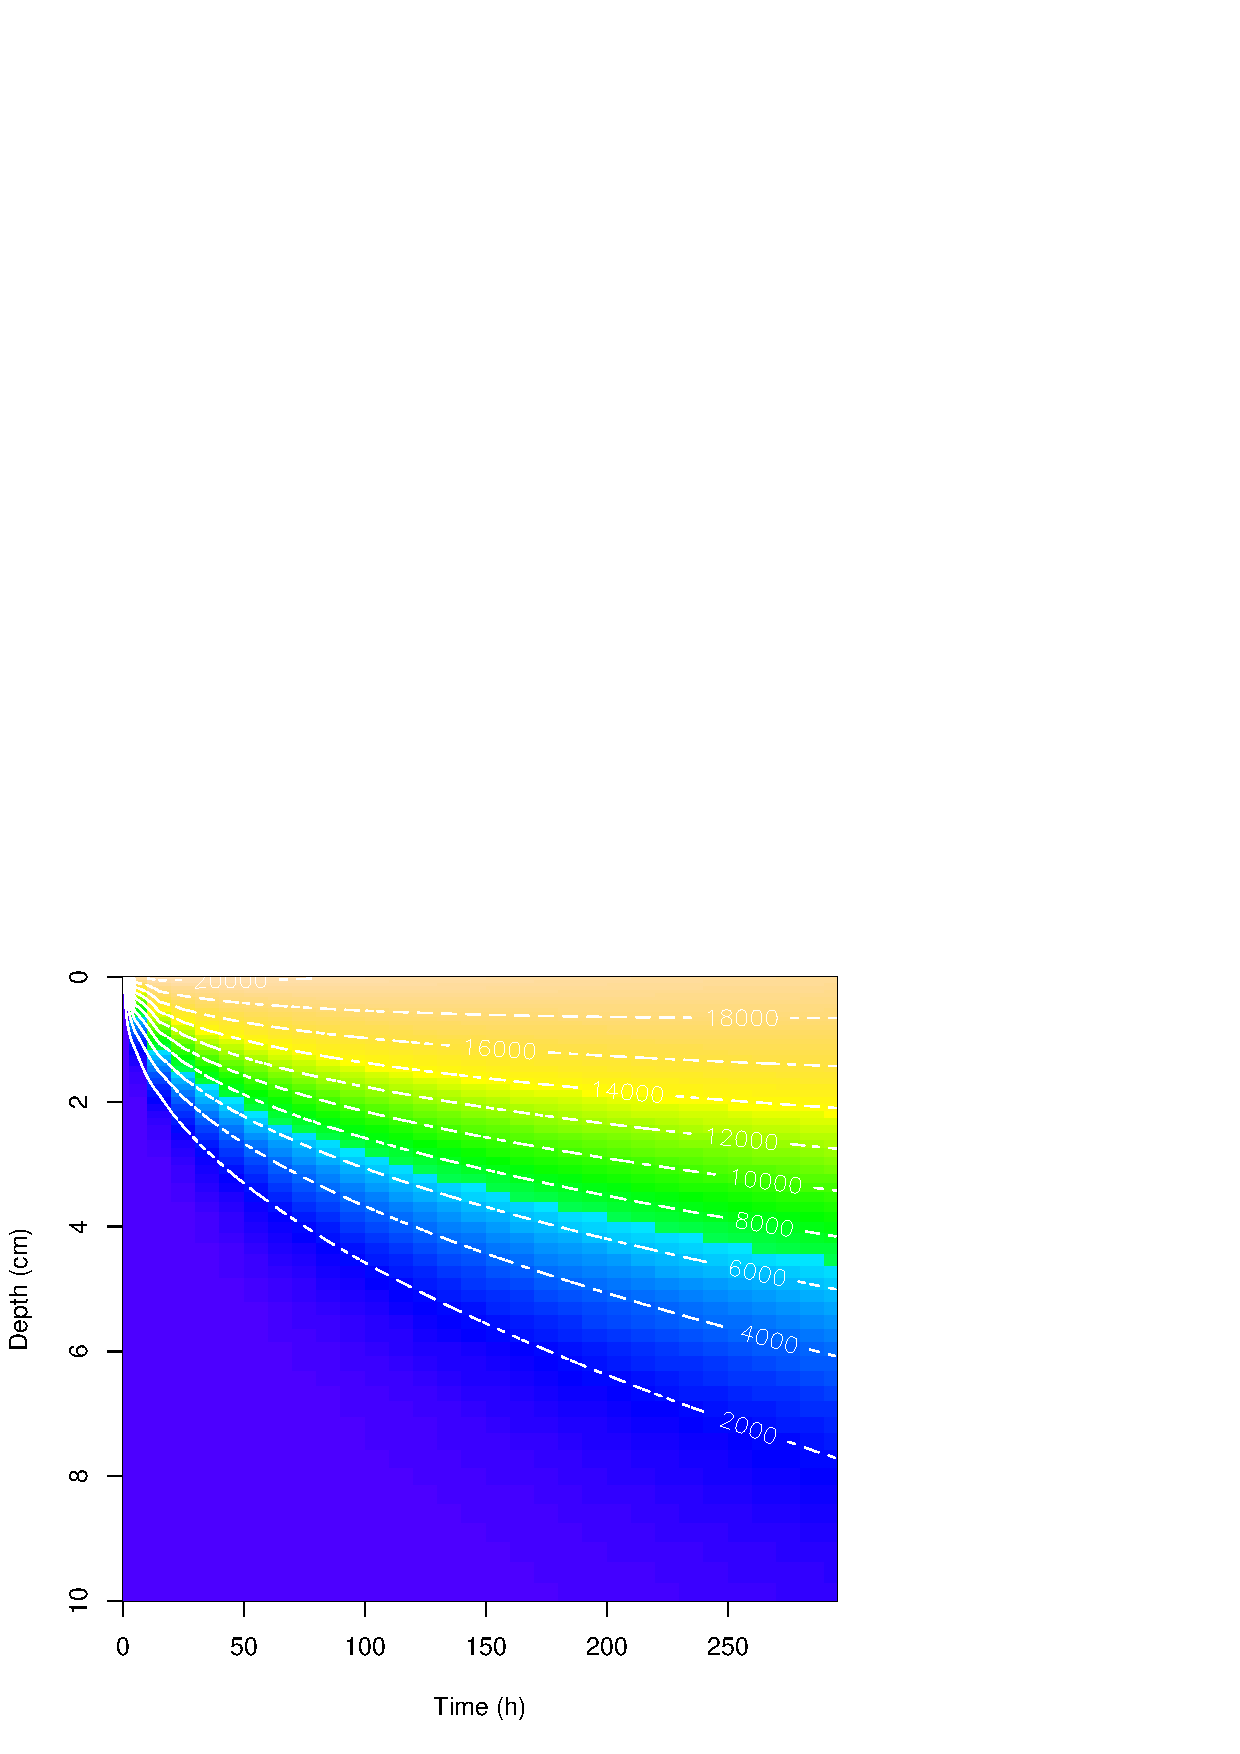
\includegraphics{figures/f-1dC}

Or if you don't like the contourlines and like other color palettes better:
\begin{Schunk}
\begin{Sinput}
> plot(test.o2, zvari = 3, ylim = c(10, 0), col = heat.colors(50), 
+     contour = FALSE)
\end{Sinput}
\end{Schunk}
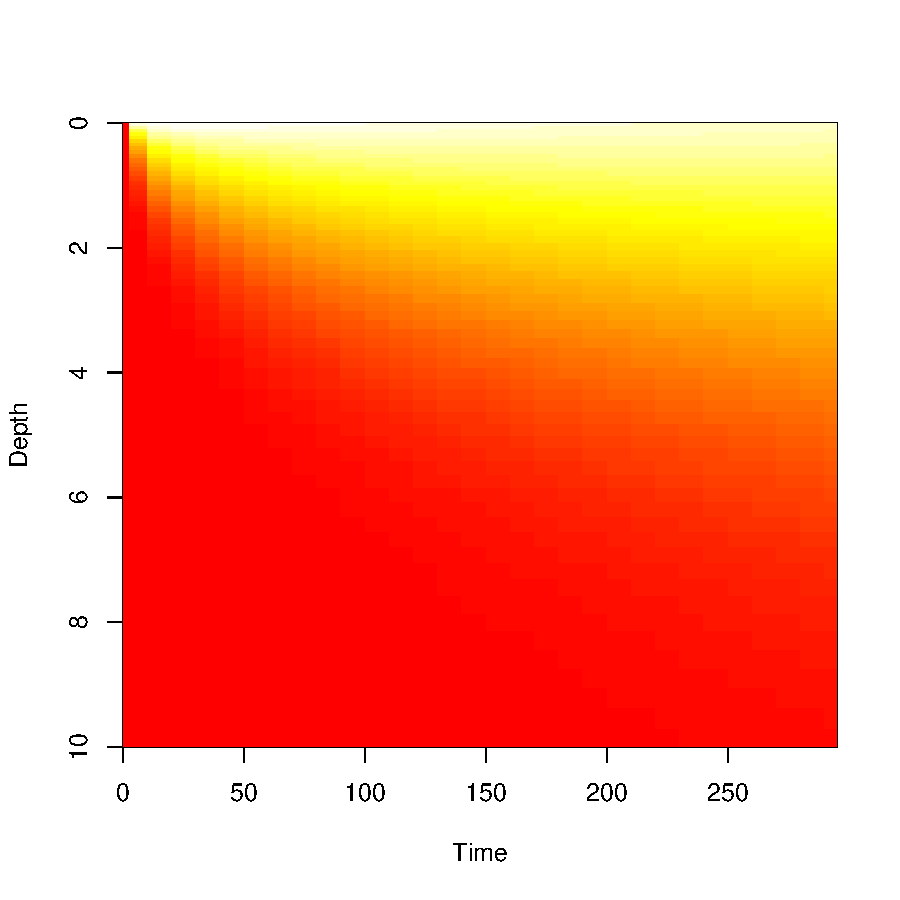
\includegraphics{figures/f-1Dd}

You can also use R functions directly:
\begin{Schunk}
\begin{Sinput}
> x <- test.o2$time
> y <- test.o2$depth
> z <- test.o2$data$TRACERSED
> persp(x, y, z, theta = 130, phi = 30, xlab = "Time", ylab = "Space", 
+     zlab = "Tracersed", shade = 0.7, main = "Model output", , 
+     col = "lightblue", border = "darkgray")
\end{Sinput}
\end{Schunk}
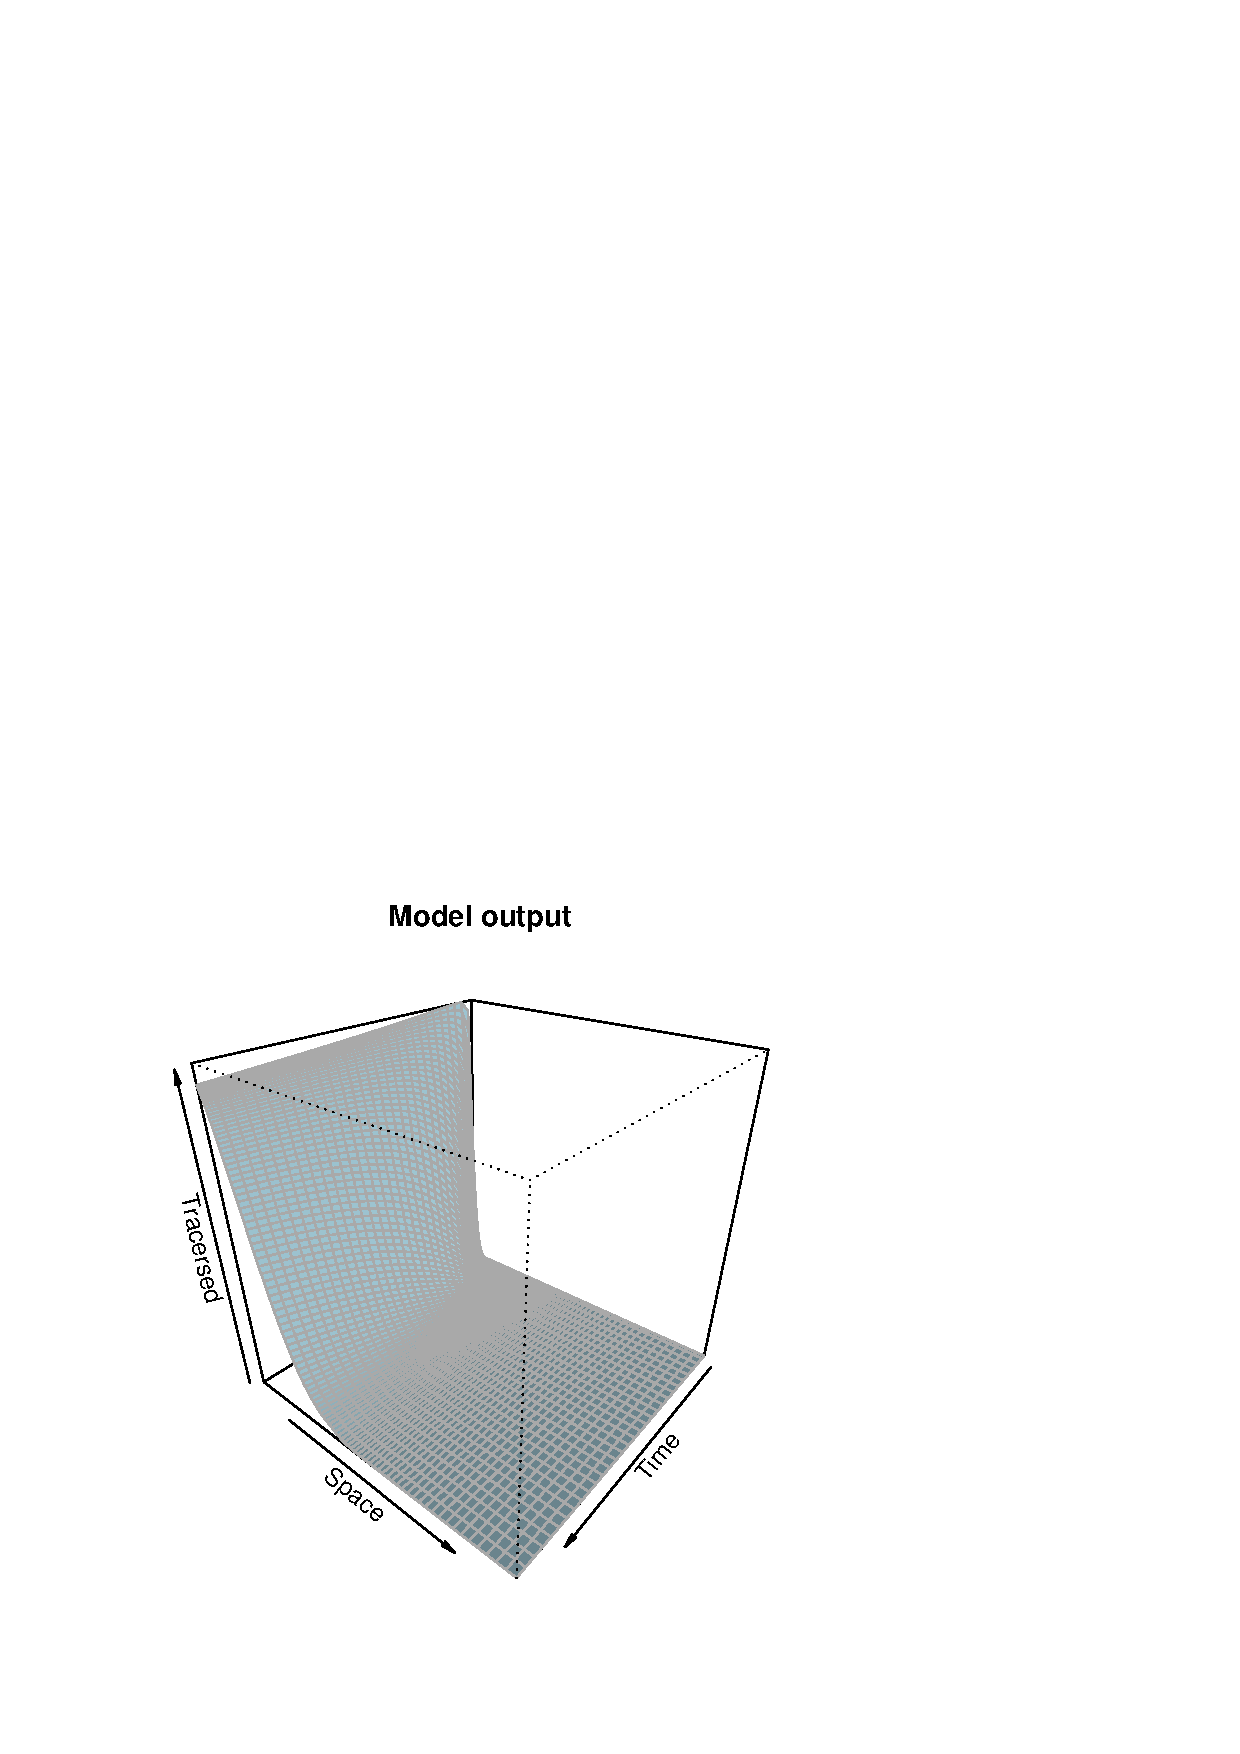
\includegraphics{figures/f-1dother}

\section{Sensitivity analysis}

Read the file and plot it \index{read.sns} \index{plot.sns}

\begin{Schunk}
\begin{Sinput}
> sensible <- read.sns("BAY2.SNS")
> plot(sensible)
\end{Sinput}
\end{Schunk}
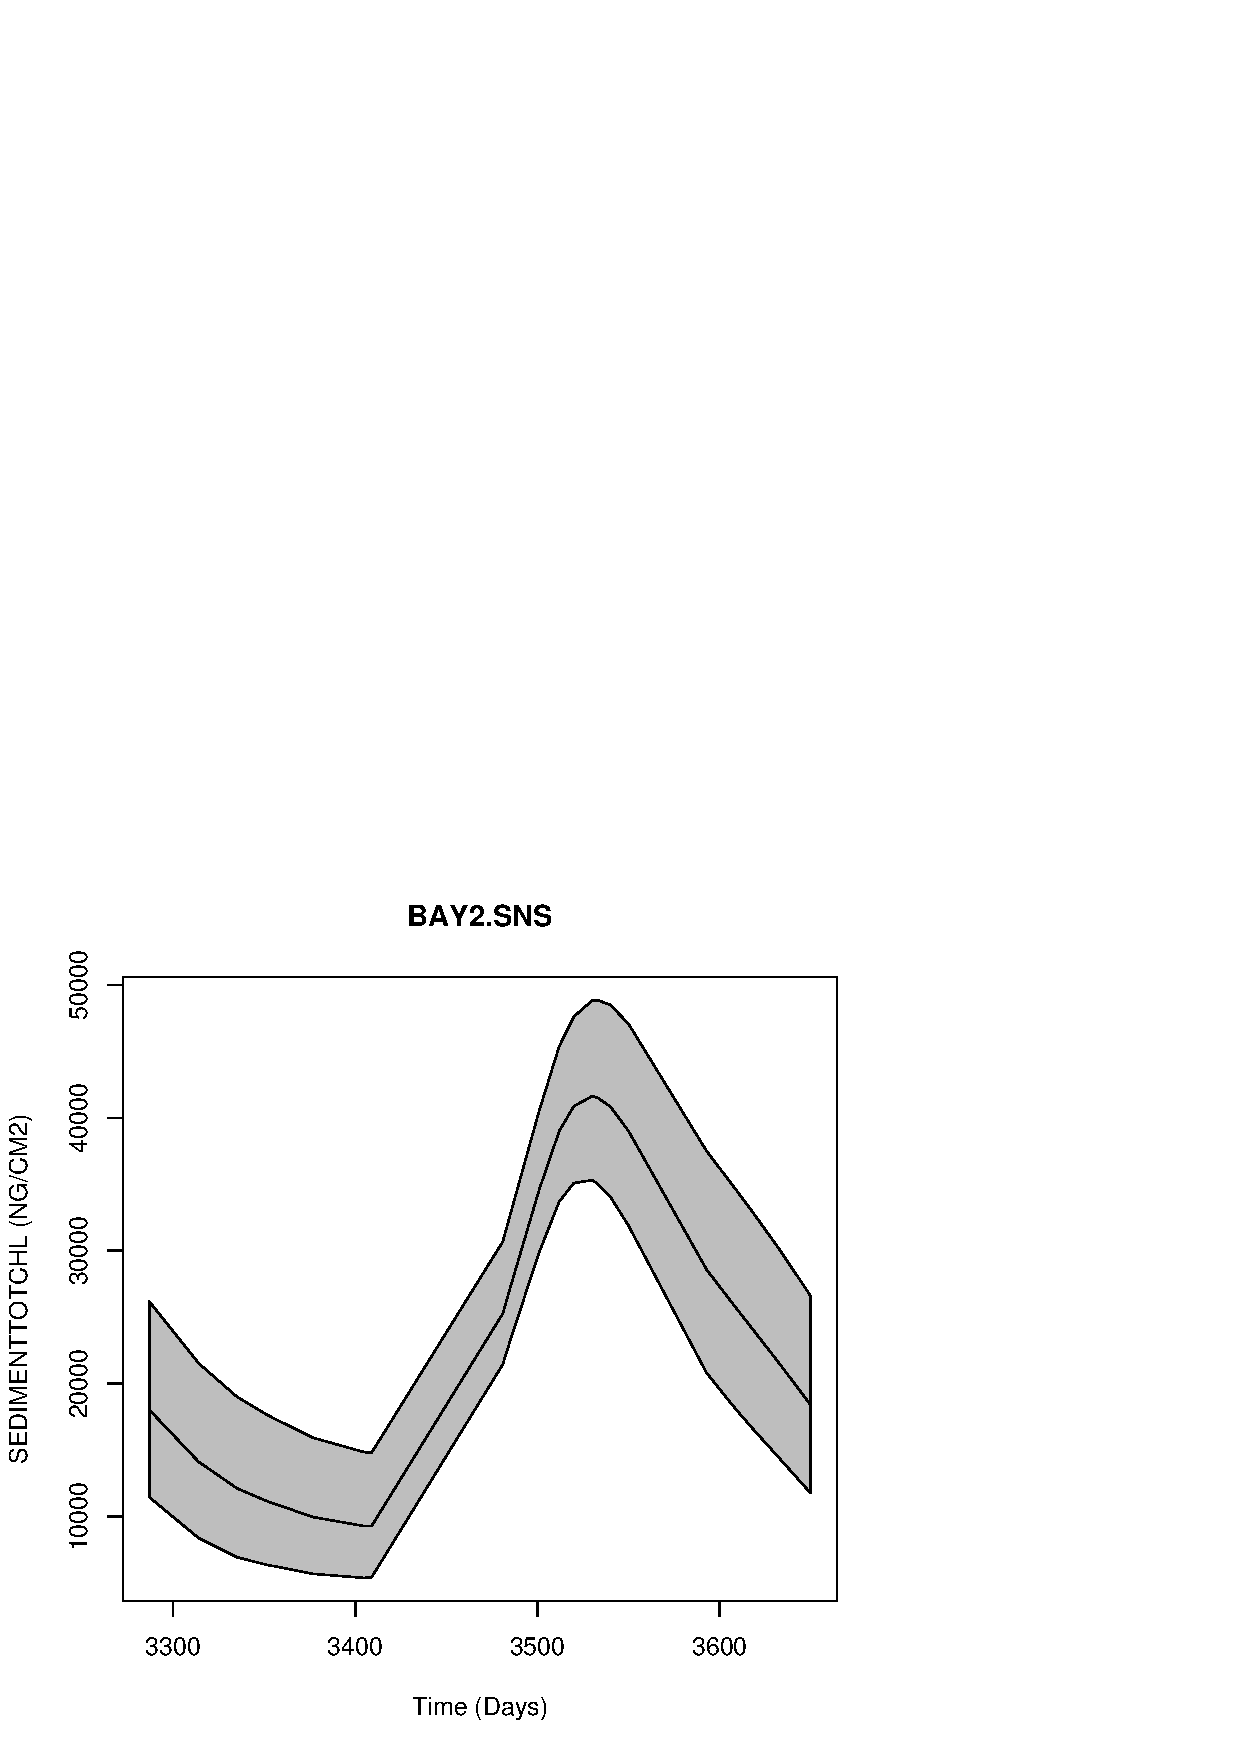
\includegraphics{figures/f-sns}

Or another variable \ldots

\begin{Schunk}
\begin{Sinput}
> plot(sensible, yvari = 6)
\end{Sinput}
\end{Schunk}
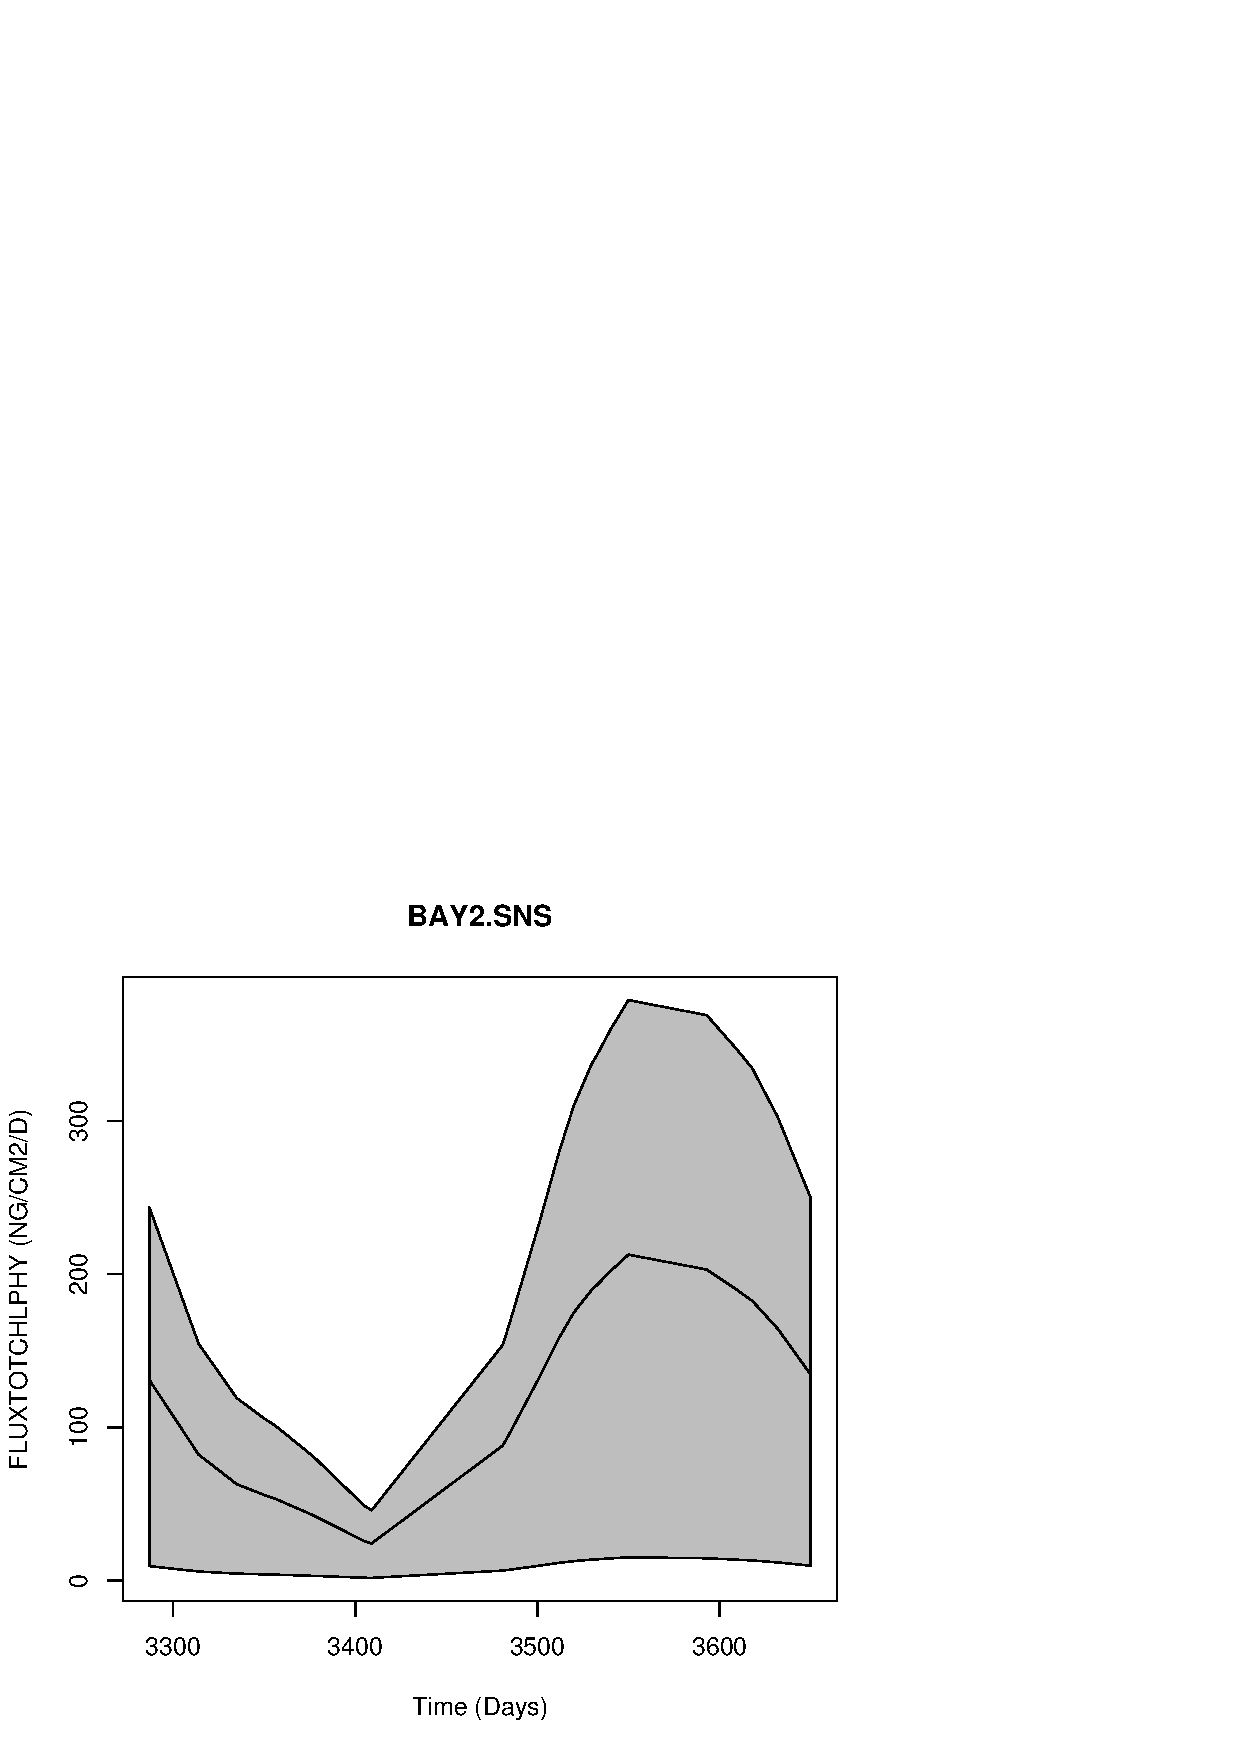
\includegraphics{figures/f-sns2}
\section{Monte Carlo simulations}
\index{read.crl}
\index{plot.crl}

\begin{Schunk}
\begin{Sinput}
> feb.crl <- read.crl("FEBRUARI.CRL")
> plot(feb.crl, xvari = 3:5, yvari = 25:28, size = 0.6)
\end{Sinput}
\end{Schunk}
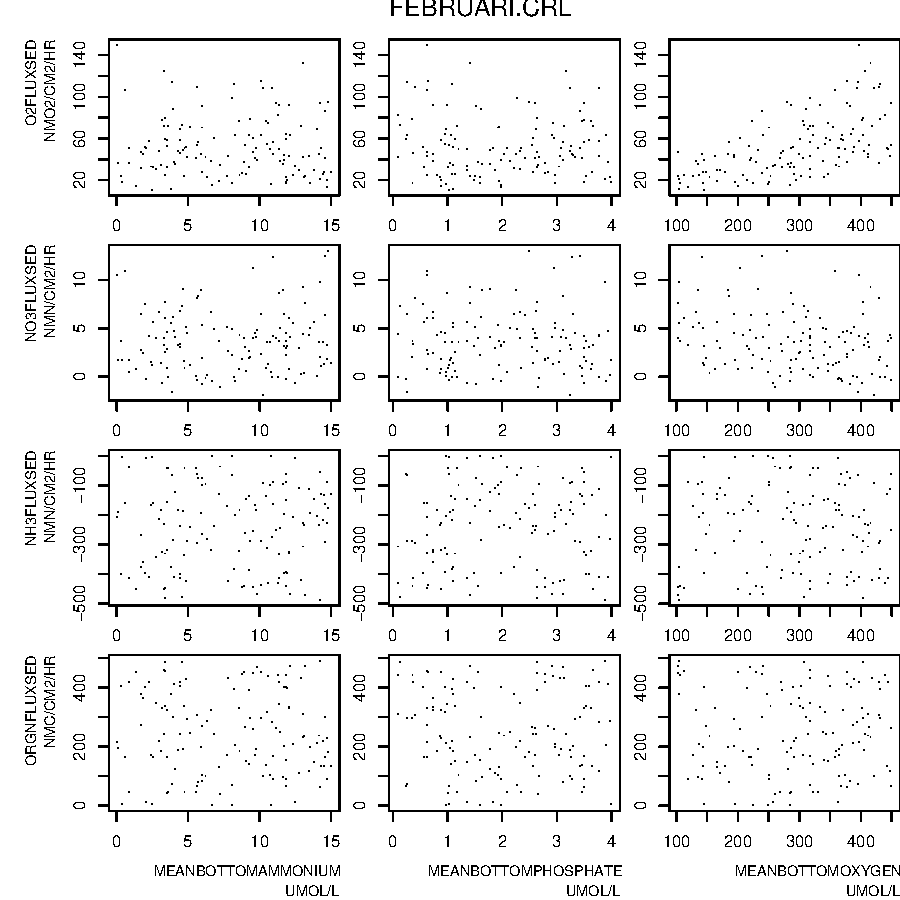
\includegraphics{figures/f-montecarlo}
\section{Parameter Covariance output analysis}


Read the file created by FEMME with
 \index{read.pcv}
\index{plot.pcv} \index{summary.pcv}


\begin{Schunk}
\begin{Sinput}
> deepradon <- read.pcv("DEEPCOLLIN.PCV")
\end{Sinput}
\end{Schunk}
Sensitivity values can be summarized using the following indexes,

\begin{align}
  \delta^{msqr}_j&
  =\sqrt{\frac{1}{n}\sum_{i=1}^n{s^2_{i,j}}}=\frac{1}{\sqrt{n}}||\mathbf{s}_j||,
  \label{eq:msqr}\\
  \delta^{mabs}_j& =\frac{1}{n}\sum_{i=1}^n{|s_{i,j}|},\label{eq:mabs}\\
  \delta^{mean}_j& =\frac{1}{n}\sum_{i=1}^n{s_{i,j}},\label{eq:mean}\\
  \delta^{max}_j& =\max_i s_{i,j},\label{eq:max}\\
  \delta^{max}_j& =\min_i s_{i,j}. \label{eq:min}
\end{align}

using,
\begin{Schunk}
\begin{Sinput}
> summary(deepradon)
\end{Sinput}
\begin{Soutput}
                        dmsqr        dmabs          mean           max
SURFACEPOROSITY  0.0132193601 0.0076389698 -0.0076389698 -5.587935e-09
MIXINGLAYER      0.0084282839 0.0036822949 -0.0036822949 -1.044571e-06
IRRIGATIONFACTOR 0.0082134266 0.0053855233 -0.0053337942  3.879685e-04
DEEPPOROSITY     0.0066735393 0.0046760328 -0.0030379979  7.975223e-03
IRRIGATIONRATE   0.0063249306 0.0050384581 -0.0050384581 -1.458824e-05
POROSITYCOEFF    0.0014904050 0.0008433500 -0.0008182440  1.882954e-04
DBCOEFF          0.0008639463 0.0004119066 -0.0004119066 -6.584451e-08
                          min
SURFACEPOROSITY  -0.031942436
MIXINGLAYER      -0.029093511
IRRIGATIONFACTOR -0.016922771
DEEPPOROSITY     -0.014398609
IRRIGATIONRATE   -0.010037018
POROSITYCOEFF    -0.003582213
DBCOEFF          -0.002560170
\end{Soutput}
\end{Schunk}
This is already done by FEMME, but using \R{} we can easily select
only a few columns or combine results from several runs,

\begin{Schunk}
\begin{Sinput}
> summary(deepradon)[, 1:2]
\end{Sinput}
\begin{Soutput}
                        dmsqr        dmabs
SURFACEPOROSITY  0.0132193601 0.0076389698
MIXINGLAYER      0.0084282839 0.0036822949
IRRIGATIONFACTOR 0.0082134266 0.0053855233
DEEPPOROSITY     0.0066735393 0.0046760328
IRRIGATIONRATE   0.0063249306 0.0050384581
POROSITYCOEFF    0.0014904050 0.0008433500
DBCOEFF          0.0008639463 0.0004119066
\end{Soutput}
\end{Schunk}
To make this into a \LaTeX{} table the \Rcode{xtable} package is useful,

\begin{Schunk}
\begin{Sinput}
> library(xtable)
\end{Sinput}
\end{Schunk}
\begin{Schunk}
\begin{Sinput}
> xtable(summary(deepradon), digits = rep(4, 6))
\end{Sinput}
% latex table generated in R 2.5.1 by xtable 1.4-3 package
% Mon Oct  1 10:34:13 2007
\begin{table}[ht]
\begin{center}
\begin{tabular}{rrrrrr}
  \hline
 & dmsqr & dmabs & mean & max & min \\
  \hline
SURFACEPOROSITY & 0.0132 & 0.0076 & $-$0.0076 & $-$0.0000 & $-$0.0319 \\
  MIXINGLAYER & 0.0084 & 0.0037 & $-$0.0037 & $-$0.0000 & $-$0.0291 \\
  IRRIGATIONFACTOR & 0.0082 & 0.0054 & $-$0.0053 & 0.0004 & $-$0.0169 \\
  DEEPPOROSITY & 0.0067 & 0.0047 & $-$0.0030 & 0.0080 & $-$0.0144 \\
  IRRIGATIONRATE & 0.0063 & 0.0050 & $-$0.0050 & $-$0.0000 & $-$0.0100 \\
  POROSITYCOEFF & 0.0015 & 0.0008 & $-$0.0008 & 0.0002 & $-$0.0036 \\
  DBCOEFF & 0.0009 & 0.0004 & $-$0.0004 & $-$0.0000 & $-$0.0026 \\
   \hline
\end{tabular}
\end{center}
\end{table}\end{Schunk}
To make a plot with default settings, type,

\begin{Schunk}
\begin{Sinput}
> plot(deepradon)
\end{Sinput}
\end{Schunk}
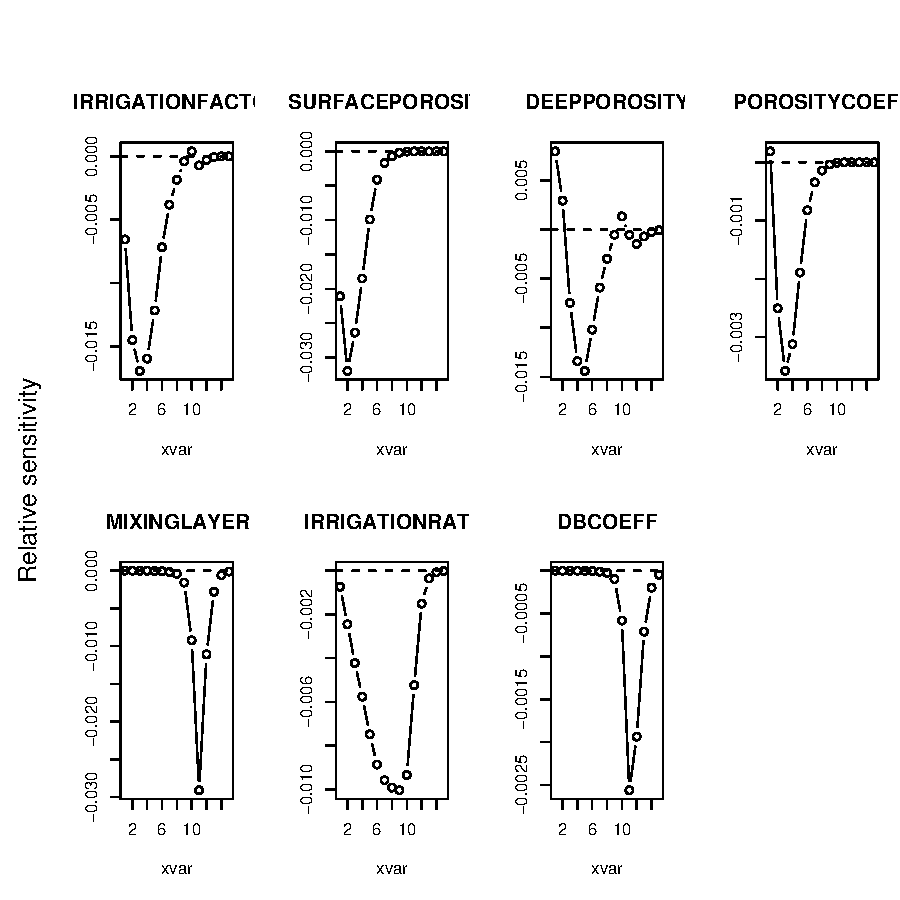
\includegraphics{figures/f-022}

It is also possible to plot only one or a selection of the parameters,

\begin{Schunk}
\begin{Sinput}
> plot(deepradon, pari = c(1, 3))
\end{Sinput}
\end{Schunk}
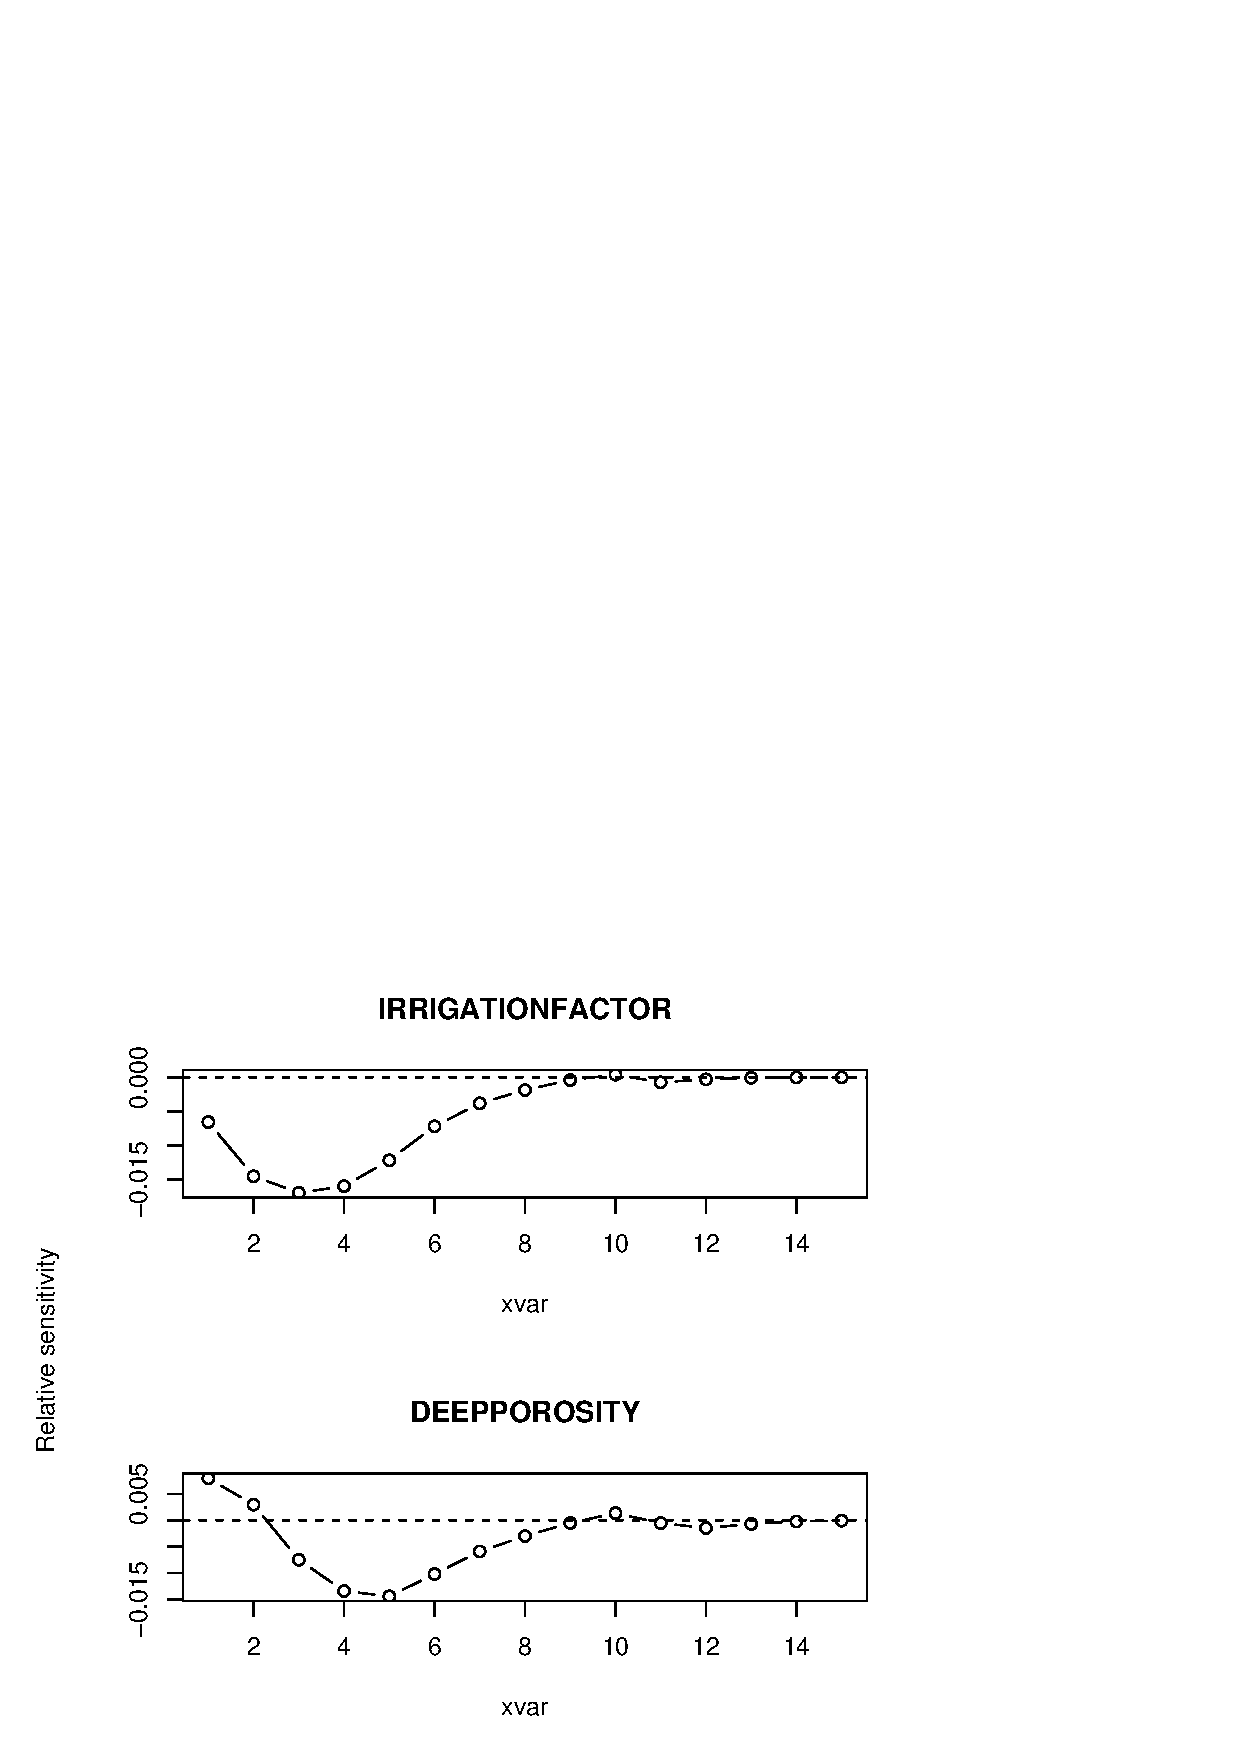
\includegraphics{figures/f-023}

Or to use a common Y-axis to get the relative importance of the
parameters in a graphical way,

\begin{Schunk}
\begin{Sinput}
> plot(deepradon, scale = TRUE)
\end{Sinput}
\end{Schunk}
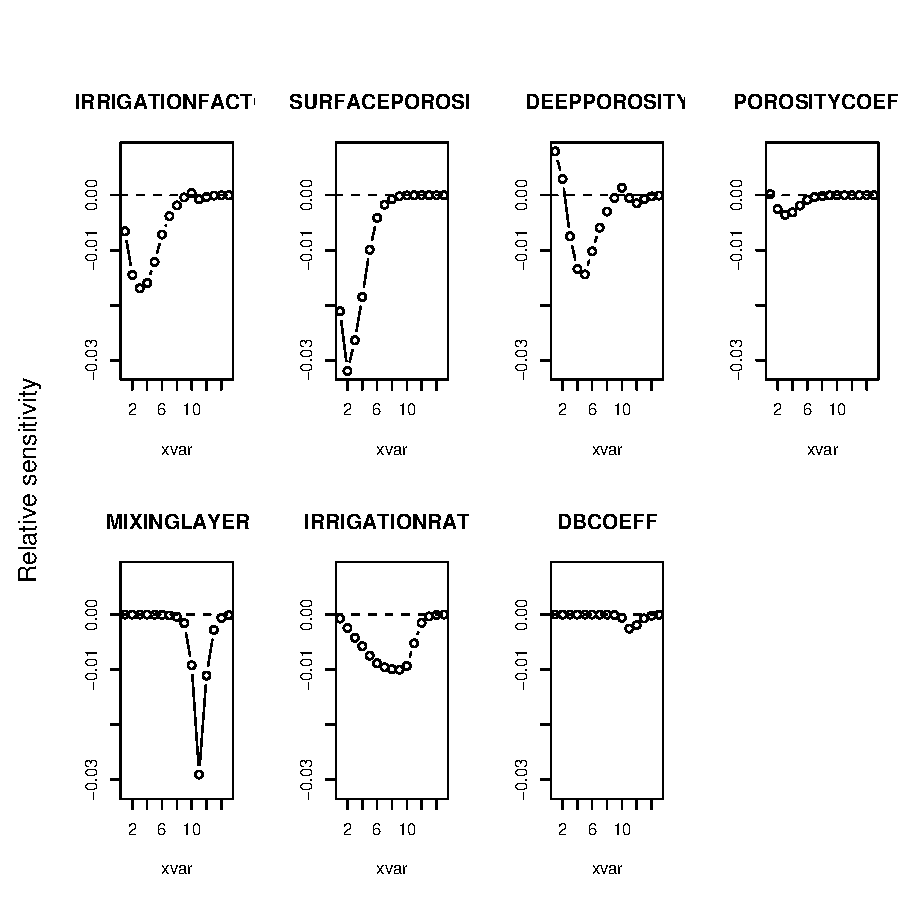
\includegraphics{figures/f-024}

For publishing quality figures you might want the parameter names to
be different than the names defined in the \Fortran{} code,

\begin{Schunk}
\begin{Sinput}
> deepradon.parnames <- c(expression(epsilon), expression(phi[s]), 
+     expression(phi[infinity]), expression(k[phi]), expression(L), 
+     expression(alpha), expression(k[alpha ~ epsilon]))
> plot(deepradon, parnames = deepradon.parnames)
\end{Sinput}
\end{Schunk}
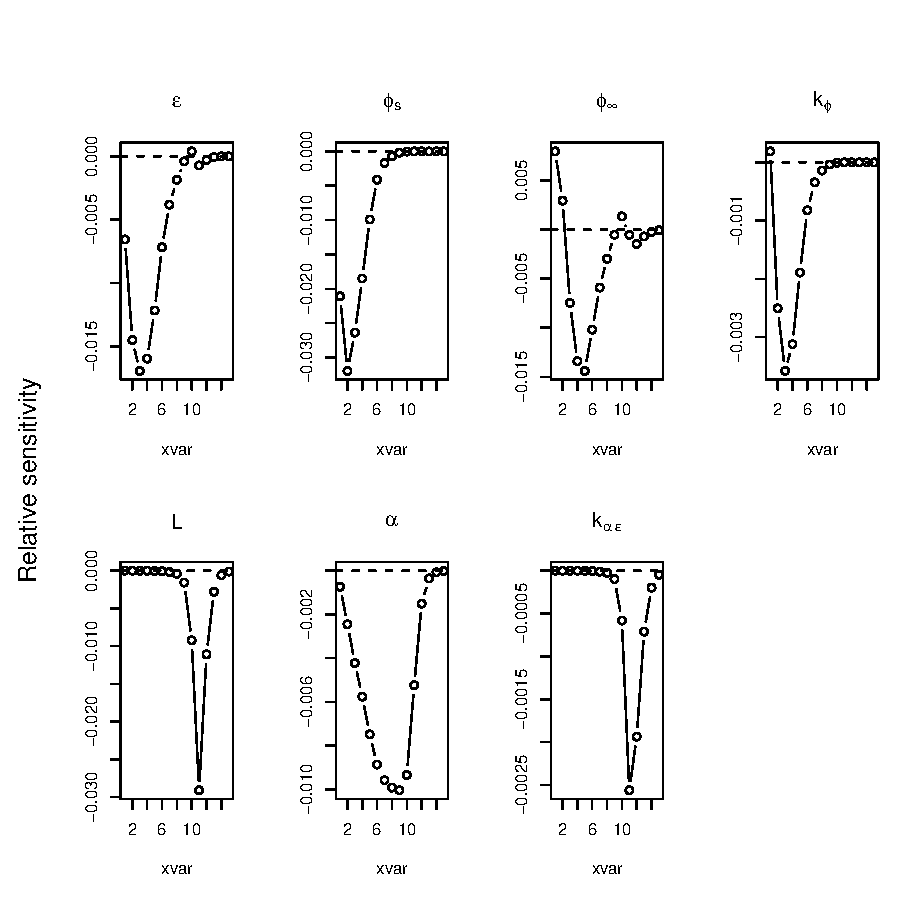
\includegraphics{figures/f-radon1}
\begin{Schunk}
\begin{Sinput}
> deepradon.parnames.tex <- c("$\\epsilon$", "$\\phi_s$", "$\\phi_\\infty$", 
+     "$k_\\phi$", "$L$", "$\\alpha$", "$k_{\\alpha,\\epsilon}$")
> xtable(summary(deepradon, parnames = deepradon.parnames.tex), 
+     digits = rep(4, 6))
\end{Sinput}
% latex table generated in R 2.5.1 by xtable 1.4-3 package
% Mon Oct  1 10:34:13 2007
\begin{table}[ht]
\begin{center}
\begin{tabular}{rrrrrr}
  \hline
 & dmsqr & dmabs & mean & max & min \\
  \hline
$\phi_s$ & 0.0132 & 0.0076 & $-$0.0076 & $-$0.0000 & $-$0.0319 \\
  $L$ & 0.0084 & 0.0037 & $-$0.0037 & $-$0.0000 & $-$0.0291 \\
  $\epsilon$ & 0.0082 & 0.0054 & $-$0.0053 & 0.0004 & $-$0.0169 \\
  $\phi_\infty$ & 0.0067 & 0.0047 & $-$0.0030 & 0.0080 & $-$0.0144 \\
  $\alpha$ & 0.0063 & 0.0050 & $-$0.0050 & $-$0.0000 & $-$0.0100 \\
  $k_\phi$ & 0.0015 & 0.0008 & $-$0.0008 & 0.0002 & $-$0.0036 \\
  $k_{\alpha,\epsilon}$ & 0.0009 & 0.0004 & $-$0.0004 & $-$0.0000 & $-$0.0026 \\
   \hline
\end{tabular}
\end{center}
\end{table}\end{Schunk}

\section{Bayesian data analysis}

Handling bayesian output is done in R by package
\Rcode{coda}~\citep{coda}. \Rcode{femmeR} only provides the ability to read a file
from Application = \femmecode{BAYES}. This creates a list with three
components, filename, vars and data, where data is the MCMC
values. \index{read.bay} 

\begin{Schunk}
\begin{Sinput}
> berg <- read.bay("BERG_END.BAY")
> summary(berg$data)
\end{Sinput}
\begin{Soutput}
Iterations = 1:2000
Thinning interval = 1 
Number of chains = 1 
Sample size per chain = 2000 

1. Empirical mean and standard deviation for each variable,
   plus standard error of the mean:

                      Mean       SD  Naive SE Time-series SE
IRRIGATIONFACTOR 2.6622577 1.663231 3.719e-02      1.494e-01
IRRIGATIONRATE   0.0007625 0.000608 1.359e-05      3.655e-05

2. Quantiles for each variable:

                      2.5%       25%      50%      75%    97.5%
IRRIGATIONFACTOR 1.0268510 1.5159075 2.123330 3.305668 7.942050
IRRIGATIONRATE   0.0000248 0.0002663 0.000626 0.001088 0.002156
\end{Soutput}
\end{Schunk}
To have a look at how the MCMC was progressing and also to get an idea
of what the posterior distribution looks like it can be visualized in
two different ways, first like this: \index{plot.bay}

\begin{Schunk}
\begin{Sinput}
> plot(berg)
\end{Sinput}
\end{Schunk}
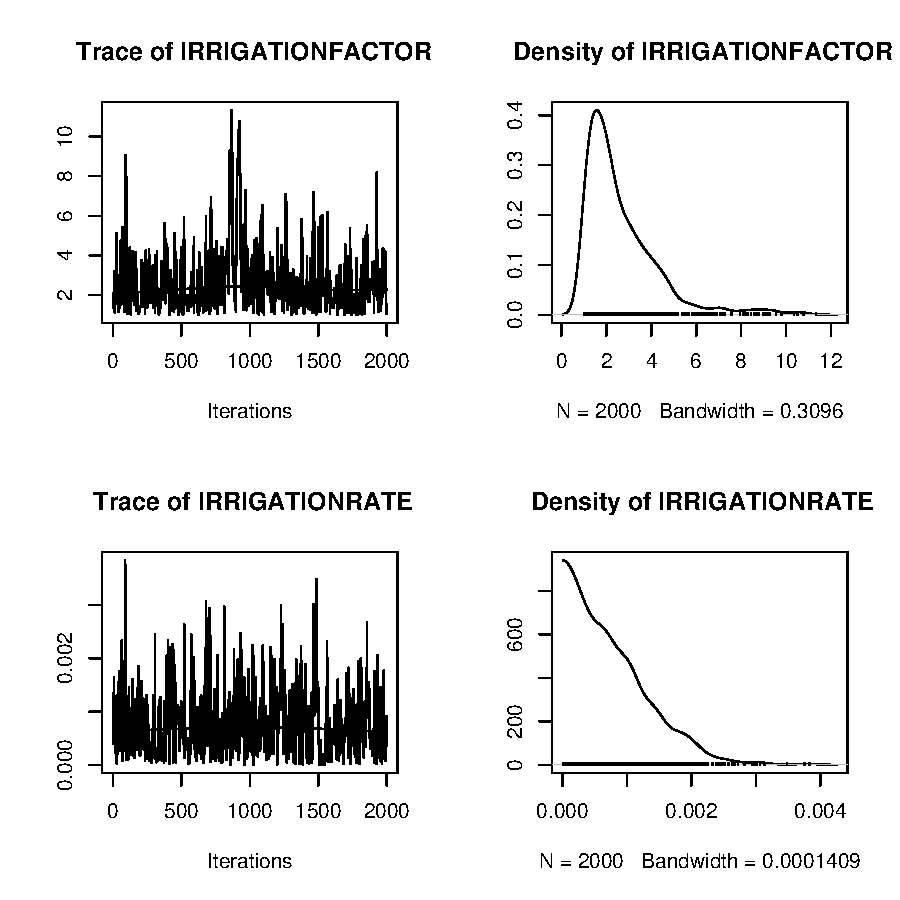
\includegraphics{figures/f-plotbay}

And secondly as a pairs plot: \index{pairs.bay}

\begin{Schunk}
\begin{Sinput}
> pairs(berg)
\end{Sinput}
\end{Schunk}
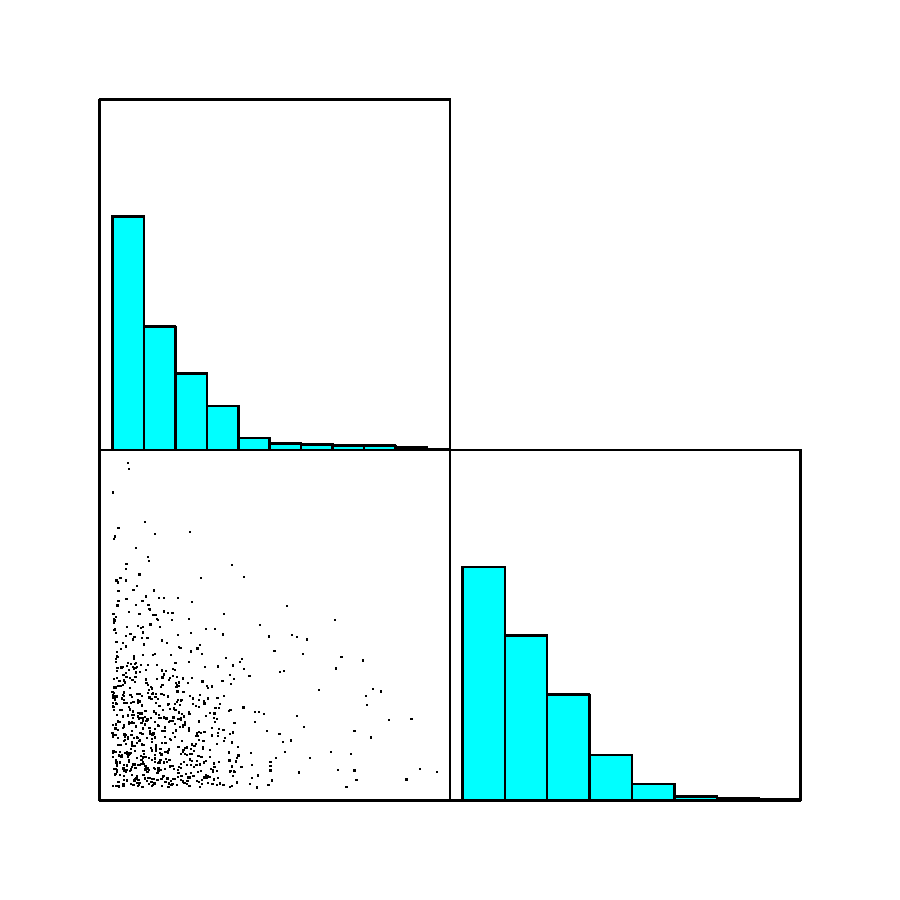
\includegraphics{figures/f-pairsbay}

To check if the MCMC simulation was run long enough we can run one of
the diagnostic utilities from \Rcode{coda}. \index{raftery.diag}

\begin{Schunk}
\begin{Sinput}
> raftery.diag(berg$data, r = 0.0125)
\end{Sinput}
\begin{Soutput}
Quantile (q) = 0.025
Accuracy (r) = +/- 0.0125
Probability (s) = 0.95 
                                                        
                  Burn-in  Total Lower bound  Dependence
                  (M)      (N)   (Nmin)       factor (I)
 IRRIGATIONFACTOR 25       4297  600          7.16      
 IRRIGATIONRATE   23       3921  600          6.54      
\end{Soutput}
\end{Schunk}
Apparently our 2000 runs are not long enough, so according to
\citet{raftery96} we tune the jumping distribution by calculating the
conditional standard deviation of the parameters multiply these with
2.3 and set this as the new jumping distribution.

\begin{Schunk}
\begin{Sinput}
> par1 <- lm(berg$data[, 1] ~ berg$data[, -1])
> summary(par1)$sigma
\end{Sinput}
\begin{Soutput}
[1] 1.650772
\end{Soutput}
\begin{Sinput}
> par2 <- lm(berg$data[, 2] ~ berg$data[, -2])
> summary(par2)$sigma
\end{Sinput}
\begin{Soutput}
[1] 0.0006034033
\end{Soutput}
\end{Schunk}

\section{Inverse analysis}

Food webs calculated by inverse analysis:

\begin{Schunk}
\begin{Sinput}
> donali <- read.web("DONALI.WEB")
> plot(donali, sizelab = 1)
\end{Sinput}
\end{Schunk}
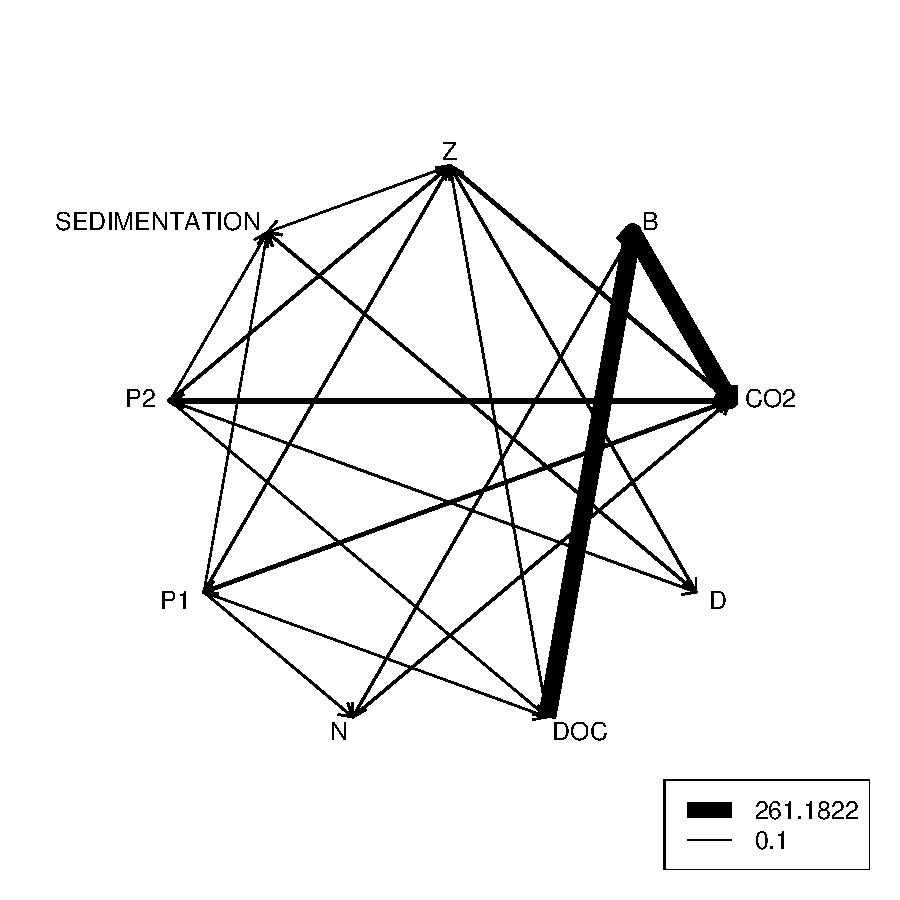
\includegraphics{figures/f-inverse}
Ranges of all flows:

\begin{Schunk}
\begin{Sinput}
> dotchart.web(donali, xlab = expression(gC ~ m^{
+     -2
+ } ~ yr^{
+     -1
+ }))
\end{Sinput}
\end{Schunk}
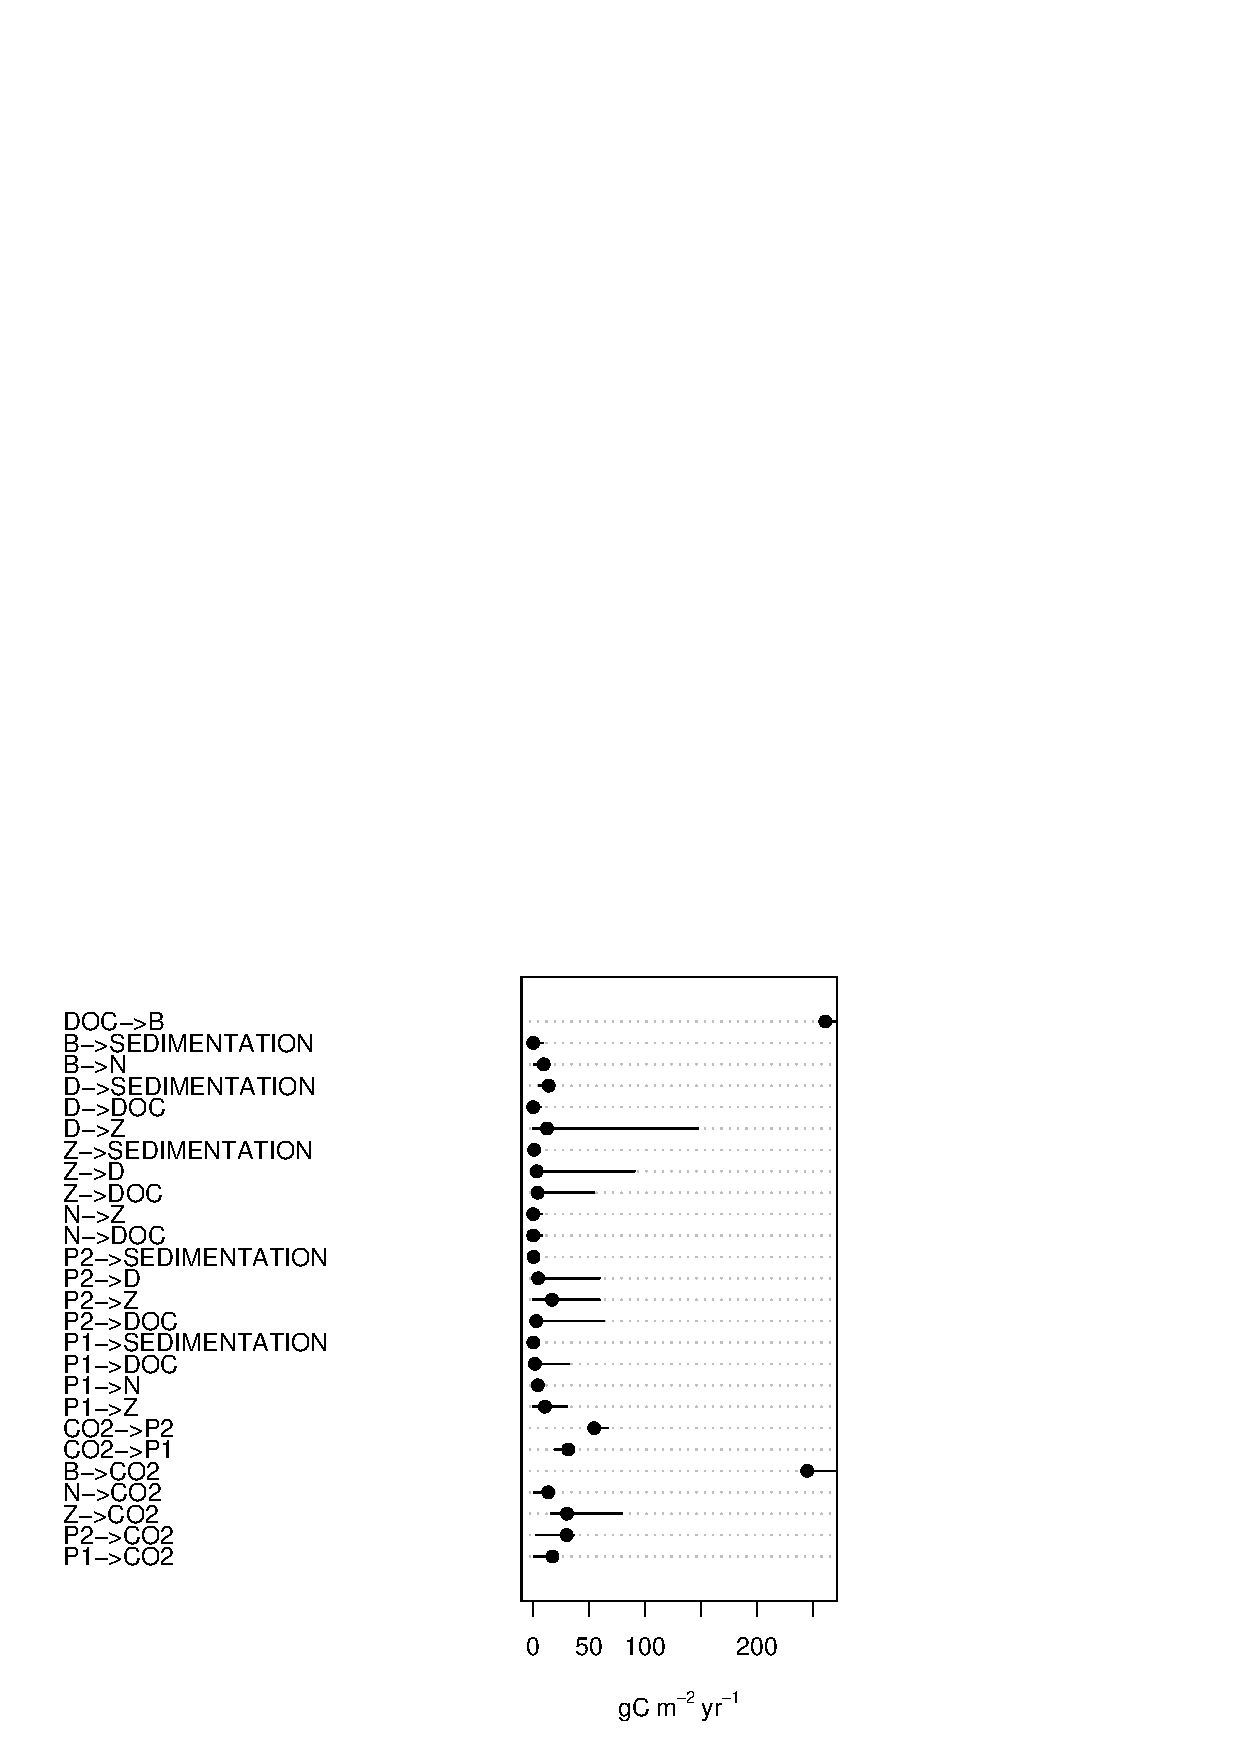
\includegraphics{figures/f-inverseranges}
\section{Parameter files}

It can be useful to be able to read and write parameter files if parameters are
varied systematically from within R and changes in model output are visualized. It can also be
useful for logging purposes. \index{read.par} \index{write.par}

\begin{Schunk}
\begin{Sinput}
> august <- read.par("august.par")
> august
\end{Sinput}
\begin{Soutput}
Parameter values for tracer model
Testing, testing           
##############
IrrigationType  =  BOTH
IrrigationFactor  =  8.13
IrrigationRate  =  4.8E-05
HeightChamber  =  0.105
SurfaceChamber  =  0.007853982
TracerAdded  =  14.43
SedimentationRate  =  0.
TemperatureChamber  =  16
SurfacePorosity  =  0.516
DeepPorosity  =  0.443
PorosityCoeff  =  0.3		
MixingLayer  =  10.
DbCoeff  =  1.
\end{Soutput}
\begin{Sinput}
> august$DeepPorosity
\end{Sinput}
\begin{Soutput}
[1] "0.443"
\end{Soutput}
\begin{Sinput}
> august[[2]] <- 5
> write.par(august, file = "")
\end{Sinput}
\begin{Soutput}
Parameter values for tracer model
Testing, testing           
##############
IrrigationType  =  BOTH 
IrrigationFactor  =  5 
IrrigationRate  =  4.8E-05 
HeightChamber  =  0.105 
SurfaceChamber  =  0.007853982 
TracerAdded  =  14.43 
SedimentationRate  =  0. 
TemperatureChamber  =  16 
SurfacePorosity  =  0.516 
DeepPorosity  =  0.443 
PorosityCoeff  =  0.3		 
MixingLayer  =  10. 
DbCoeff  =  1. 
\end{Soutput}
\begin{Sinput}
> write.par(august, file = "test.par", ask = FALSE)
\end{Sinput}
\end{Schunk}

\textbf{Please note that using write.par with file set to something
  else than "" and ask=F, will overwrite existing files with the same
  name without asking before}

\newpage 
\appendix
\section{A short introduction to R}
\label{sec:short-introduction-r}


\subsection{Using packages e.g. \Rcode{femmeR}}

To load packages for \R{} use the command \fn{library} and to load
\Rcode{femmeR} assuming you haven't done it already use \texttt{library(femmeR)}


\subsection{Working directory}

To see which directory you are currently working in, use \fn{getwd}
and to change it use \fn{setwd}. Just remember to use forward slashes
separating the directory names.

If you work with different projects in some folders on your computer
you can also use the \fn{.Rdata} file which is saved at the end of the
session if you answer yes on ``Save workspace image''. Doubleclick the
\texttt{.Rdata} and \R{} will start up in that folder and your previous
workspace is restored.

\subsection{Getting help}
\label{sec:getting-help}

To get help about a function use \texttt{?function} e.g \texttt{?plot}
gets you all the information about scatter plots. If you don't know
the name of the function, try \mbox{\texttt{help.search("useful
    phrase")}}. To read the \Rcode{femmeR} manual use
\texttt{vignette("femmeR")}.

\subsection{Entering data}
\label{sec:data}

To create a vector use the command \fn{c}.
\begin{Schunk}
\begin{Sinput}
> n = c(1, 5, 7)
> n
\end{Sinput}
\begin{Soutput}
[1] 1 5 7
\end{Soutput}
\end{Schunk}
Some examples of sequences:

\begin{Schunk}
\begin{Sinput}
> x = 1:10
> x
\end{Sinput}
\begin{Soutput}
 [1]  1  2  3  4  5  6  7  8  9 10
\end{Soutput}
\begin{Sinput}
> y = seq(0, 1, length = 11)
> y
\end{Sinput}
\begin{Soutput}
 [1] 0.0 0.1 0.2 0.3 0.4 0.5 0.6 0.7 0.8 0.9 1.0
\end{Soutput}
\begin{Sinput}
> F = rep("A", 2)
> F
\end{Sinput}
\begin{Soutput}
[1] "A" "A"
\end{Soutput}
\end{Schunk}
Combining them:

\begin{Schunk}
\begin{Sinput}
> G = rep(c("A", "B"), 3)
> G
\end{Sinput}
\begin{Soutput}
[1] "A" "B" "A" "B" "A" "B"
\end{Soutput}
\end{Schunk}
\subsection{Subplots}
\label{sec:subplots}

\begin{Schunk}
\begin{Sinput}
> par(mfrow = c(1, 2))
> plot(nh4, z, type = "b")
> boxplot(heffa ~ f)
\end{Sinput}
\end{Schunk}
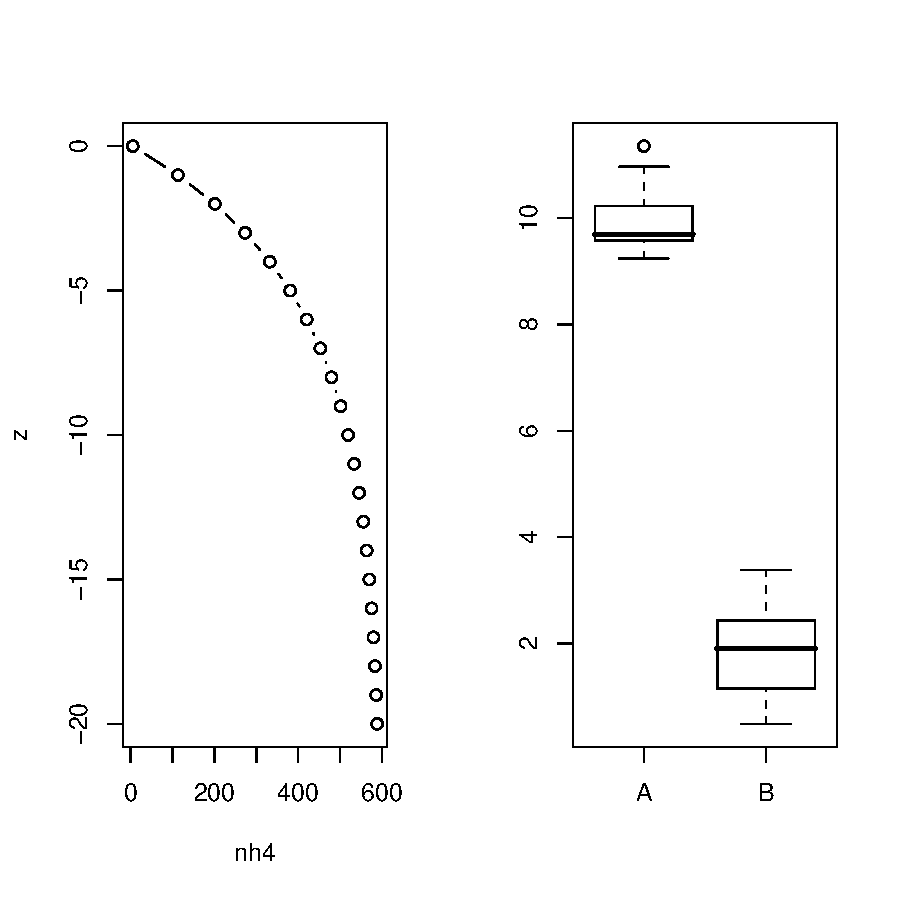
\includegraphics{figures/f-subplot}

\subsection{Mathematical expressions}
Here is a short example with some sub/super-scripts. To get more
information, try \Rcode{demo(plotmath)}.


\begin{Schunk}
\begin{Sinput}
> x <- seq(0, 10, length = 100)
> y <- 20/x + x^2
> curve(20/x + x^2, xlim = c(0, 10))
> title(main = expression(frac(20, x) + x^2))
> text(5, 100, expression(C[2] * H[4] + 3 ~ O[2] %->% 2 ~ H[2] * 
+     O + 2 ~ CO[2]))
\end{Sinput}
\end{Schunk}
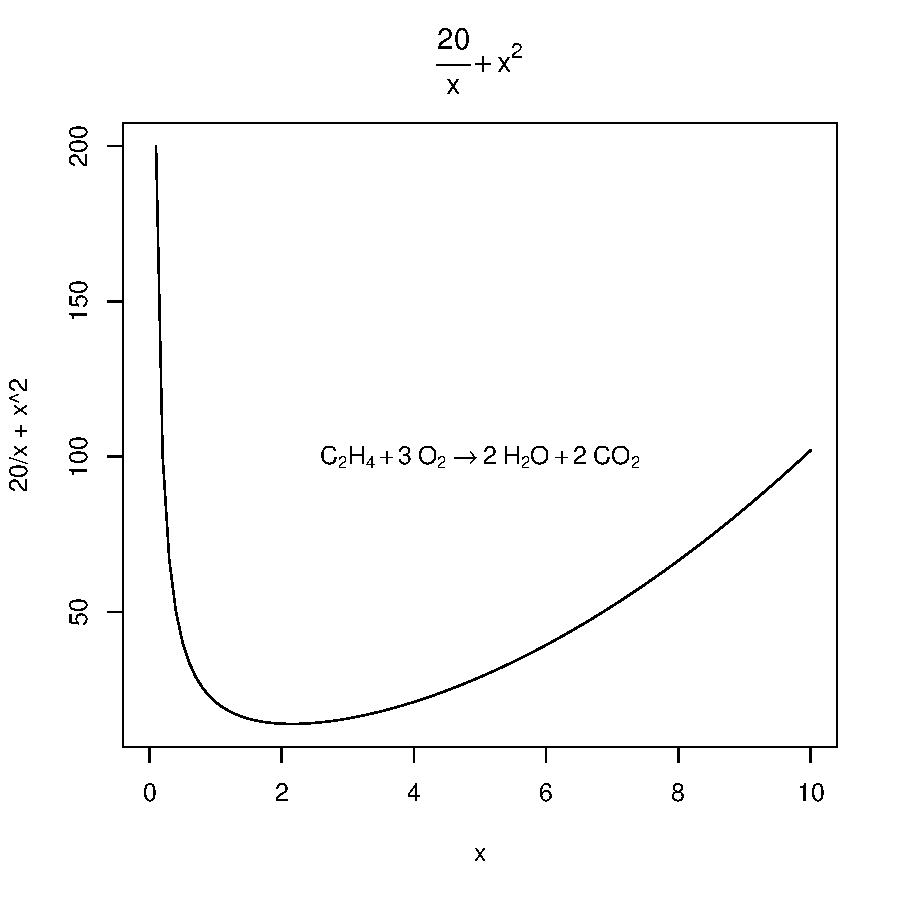
\includegraphics{figures/f-math1}

\subsection{Customizing plots}

To find possible changes to make to a plot look at \Rcode{?par}. 

\begin{Schunk}
\begin{Sinput}
> plot(test, yvari = 2, main = "")
> abline(v = 12, lty = 2, col = 2)
> text(15.1, 0.1, "Mixed layer depth", adj = 0)
> arrows(15, 0.1, 12, 0.12, lwd = 2)
\end{Sinput}
\end{Schunk}
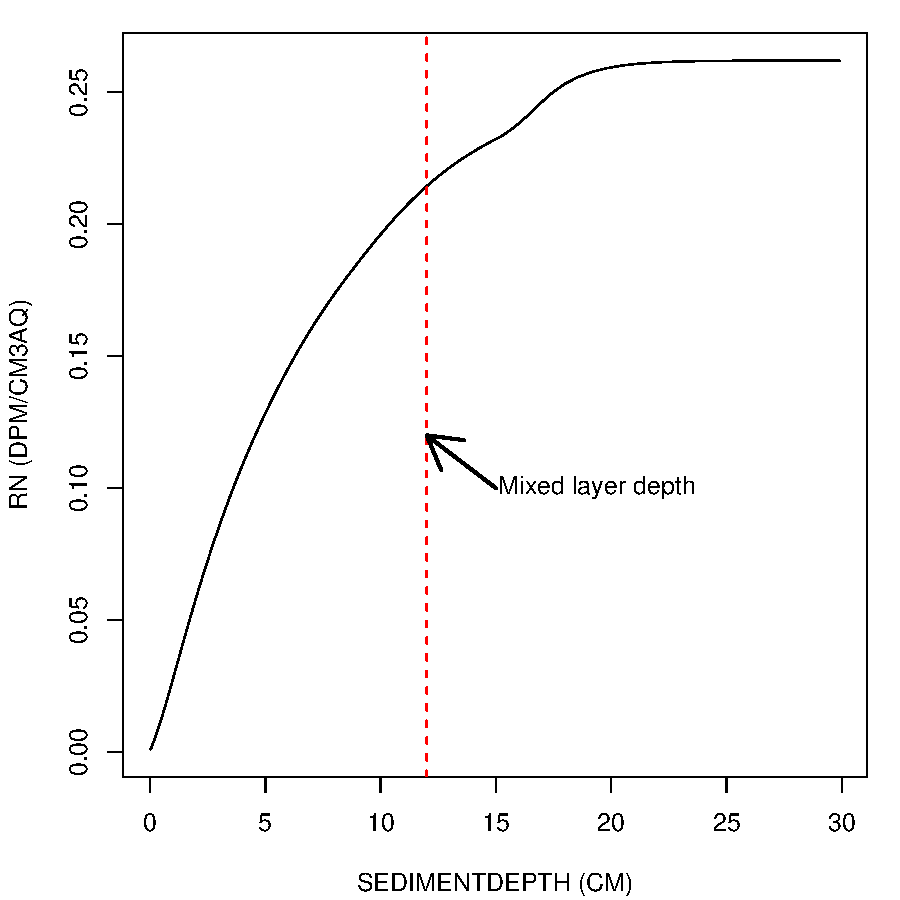
\includegraphics{figures/f-margins}
\subsection{Using colors}
If you make a graph intended for a poster or presentation, using
colors can be very helpful and also makes your graphs look more
interesting.

You can use colors by their name e.g. ``green'' or by hexadecimal
notation. The latter is best generated by specialized functions such
as \texttt{rainbow}.

\begin{Schunk}
\begin{Sinput}
> par(mfrow = c(2, 2))
> barplot(rep(c(1, 2), 5), col = rainbow(2))
> barplot(rnorm(5), col = heat.colors(5))
> barplot(1:10, col = rainbow(10))
> pie(1:10, col = terrain.colors(10))
\end{Sinput}
\end{Schunk}
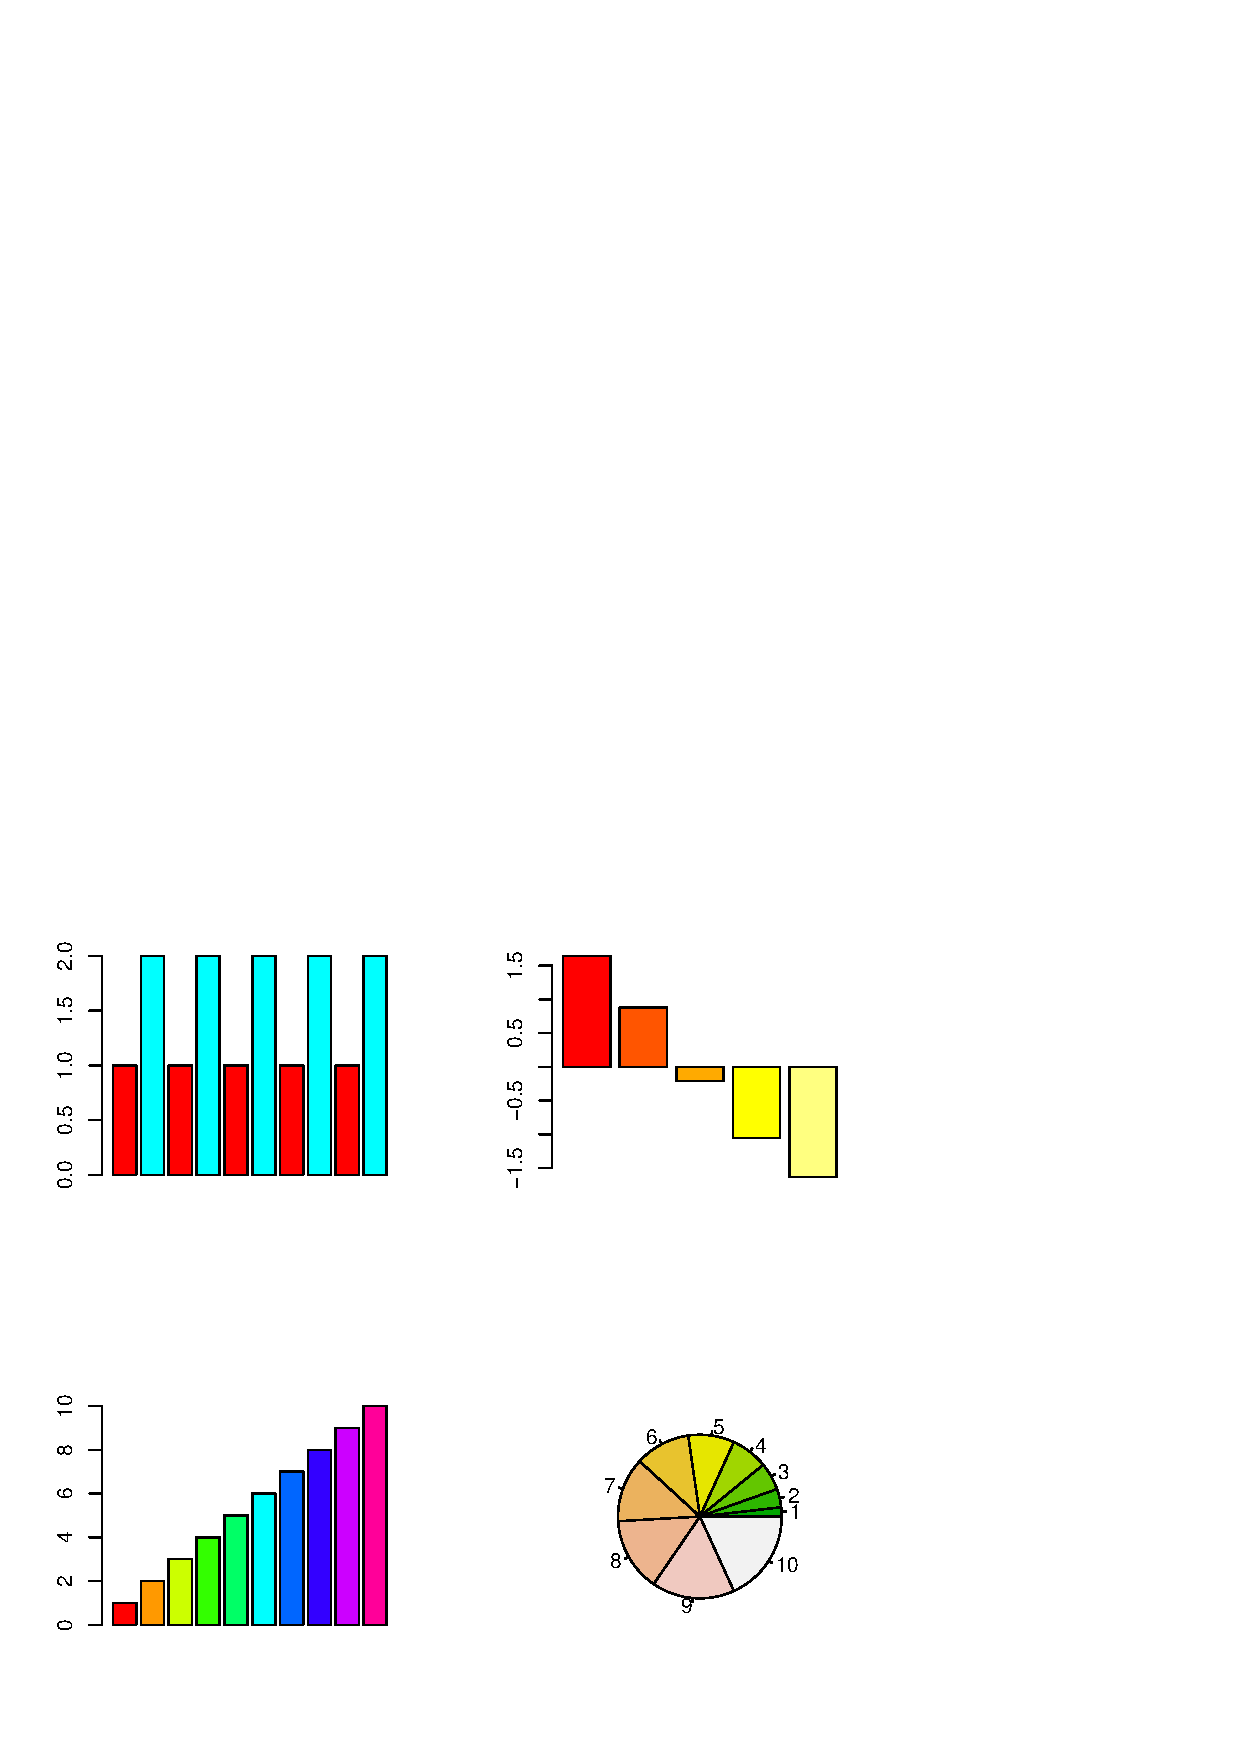
\includegraphics{figures/f-042}
\bibliography{R}
\bibliographystyle{plainnat}

\printindex

%% ------------------------------------------------------------------
\end{document}
